\chapter{람다계산법과 하스켈}
앞으로 이 책에서는 문법구조, 의미구조 등 프로그래밍언어에 관한
개념을 직접 하스켈(Haskell) 코드로 작성해 보는 실습과 함께
조금 더 구체적으로 알아볼 것이다. 하스켈은 람다계산법에 기반한
순수 함수형 프로그래밍언어로 게으른 값계산(lazy evaluation)에
따라 실행되며 타입 유추(type inference)를 지원하는 강력한
정적 타입 시스템을 갖추고 있다. 여기서는 하스켈 컴파일러인
GHC를 주피터(Jupyter) 환경에서 사용하게 해 주는 IHaskell 커널을
도커 이미지로 포장한 ihaskell-notebook\footnote{%
\url{https://github.com/IHaskell/ihaskell-notebook}}을 기준이 되는
실습 환경으로 한다. 인쇄된 교재 및 교재 Github 홈페이지\footnote{%
\url{https://github.com/hnu-pl/PLbook}}를 통해 제공되는
모든 하스켈 코드 예제를 이 환경에서 직접 실행해 볼 수 있다.
부록 \ref{sec:codespace}를 참고하여 교재 Github 홈페이지에서
미리 설정해 놓은 프로그래밍 환경을 Github Codespaces를
활용해 구동하는 것을 권장한다.

이 장에서는 하스켈 언어의 기원에 대해 간단히 소개한 다음,
람다계산법과 관련지어 하스켈을 이해하도록 설명한다.
설명과 곁들인 하스켈 주피터 노트북 환경에서 실행되는 예제를 통해
하스켈 언어의 기본적인 개념과 문법, 또 앞으로 계속 사용하게 될
이 프로그래밍 환경과도 친숙해지기로 한다.
\newpage

\begin{figure}\centering
\begin{subfigure}[b]{.3\textwidth}\centering
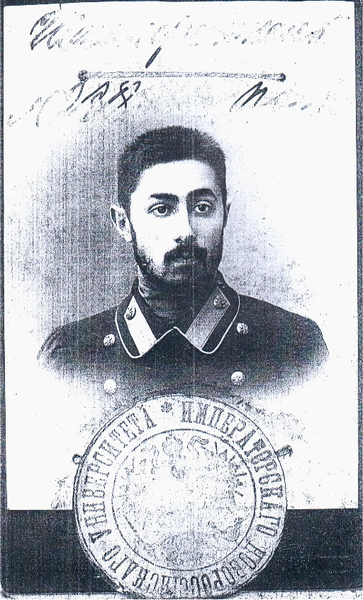
\includegraphics[trim={70pt 250pt 80pt 110pt},clip,scale=.9]{Schonfinkel.png}
\caption{Moses Sch\"onfinkel}
\end{subfigure}
\begin{subfigure}[b]{.3\textwidth}\centering
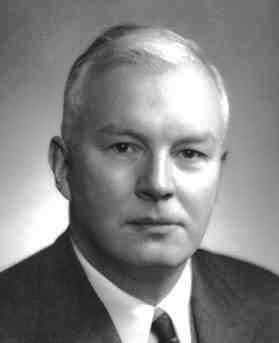
\includegraphics[scale=.8]{HaskellBCurry.jpg}
\caption{Haskell Curry}
\end{subfigure}
%\haskelllogo
\caption{조합논리(conbinatory logic)의 창시자인
         모지스 쇤핑클과 이를 체계화한 하스켈 커리
         {\footnotesize(사진 출처: 위키미디어 공용)} }
\end{figure}

\section{하스켈 프로그래밍언어의 기원}
`하스켈'이라는 프로그래밍언어의 이름은 조합논리(combinatory logic)를
정립한 하스켈 커리의 이름을 따른 것이다. 하스켈이 함수형 프로그래밍언어라고
이 장의 첫머리에서 앞서 언급했는데, 함수형 언어가 무엇인지 아주 간단히
이야기하자면 람다계산법에 기반을 둔 프로그래밍언어의 부류라 할 수 있다.
그렇다면 왜 람다계산법의 창시자인 알론조 처치의 이름을 따라 `알론조'라 부르지
않았냐면 아마도 이미 선점\cite{Ramsdell1989alonzo}되었기 때문인 것 같다.
어디까지나 추측이지만 만일 선점되지 않았더라면 하스켈이 아닌 알론조라고
지었을 가능성도 있을 것 같다. 이왕 주제를 벗어난 김에 흥미로운 일화를 하나
소개하자면, 알론조 처치의 아들은 (본인의 말에 따르면) 하스켈 커리의 딸과
사귄 적이 있었다고 한다.\footnote{%
\url{https://importantshock.wordpress.com/2007/08/21/haskell-curry-yes-i-dated-his-daughter/}}

다시 하스켈의 역사\cite{Hudak2007HistoryHaskell} 이야기로 돌아오면,
하스켈은 학계의 효율적인 연구 활동을 위해 학계에서 위원회를 구성해 만든 언어다.
1980년대 후반 즈음에는 게으른 값계산에 따라 실행되는 정적 타입을 갖춘
함수형 프로그래밍언어에 대해 연구하던 사람들이 각자 자신의 연구를 위해
비슷한 기능을 가진 학술 연구를 위한 실험용 언어를 중구난방으로 만들고
있던 상황이었다고 한다. 그래서 비슷한 주제에 관심을 가진 연구자들끼리
같이 쓸 수 있는 하나의 언어를 정의하면 서로 문법을 다르게 정의한 예제
코드를 포함한 논문을 읽어야 하는 소통의 부담도 줄이고 구현에 드는 중복된
노력도 덜 수 있으리라는 희망으로 새로운 언어를 만드는 위원회를 시작한 것이
그 기원이라고 한다.

사공이 많으면 배가 산으로 간다는 속담처럼 위원회가 만드는 언어는,
특히나 학계의 위원회라면, 그 위원회가 활동하는 동안에만 연구논문을
위한 실험적 용도로만 쓰다 이후에 다른 곳에는 아무도 쓰지 않는 것이 보통이며,
설령 그렇더라도 충분히 의미있는 경우도 있다. 예를 들어 ALGOL이 대표적으로
학계 위원회의 언어인데, 그 자체로는 업계에서 활발히 도입되지 않았겠지만
이후의 프로그래밍언어 설계 패러다임을 바꿀 만큼, 특히 GOTO를 버리고
구조적 프로그래밍을 지원하는 것이 당연시되도록, 지대한 영향을 미쳤다.
하스켈은 학계의 연구용 언어로서도 성공을 거뒀을 뿐 아니라 업계에서도
(C++, Java, Python, JavaScript 급의) 주류 개발 언어는 아니지만 여러
리눅스 배포판에 패키지가 안정적으로 제공되며 최근에는
블럭체인\cite{Seijas2020Marlowe} 등 다양한 영역에서 활용되고 있다.

\begin{figure}\centering
\begin{subfigure}{.3\textwidth}\centering
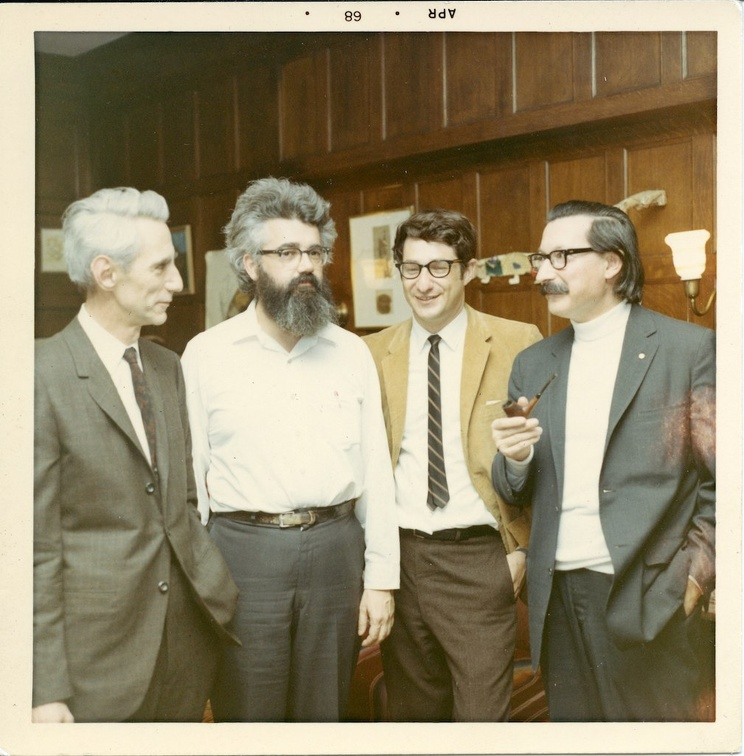
\includegraphics[trim={200pt 380pt 380pt 175pt},clip,scale=.8]{ShannonMcCarthyFredkinWeizenbaum.jpg}
\caption{John McCarthy}
\end{subfigure}
\qquad\qquad
\begin{subfigure}{.3\textwidth}\centering
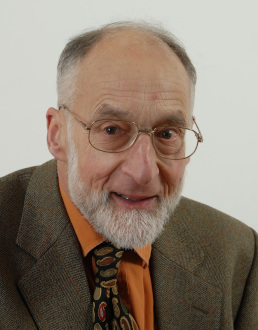
\includegraphics[trim={0 20pt 0 0},clip,scale=.8]{RobinMilner.jpg}
\caption{Robin Milner}
\end{subfigure}
\caption{LISP의 창시자이자 인공지능의 아버지인 존 매카시,\\
         ML과 파이계산법($\pi$-calculus)의 창사자인 로빈 밀너\\
         {\footnotesize(사진 출처: \texttt{media.csail.mit.edu},
                        위키미디어 공용)}
	 \label{fig:McCarthyMilner} }
\end{figure}

\index{함수형 언어|see{functional language}}%
\index{functional language|see{함수형 언어}}%
더 역사를 거슬러 올라가 보면 존 매카시가 최초의 함수형 언어로 볼 수 있는
\index{함수형 언어!리습}
\index{functional language!LISP}
\index{리습|see{LISP}}%
\index{LISP|see{리습}}%
리습(LISP)을 1950년대 말에 만들었고, 로빈 밀너의 주도로 타입 유추를
지원하는 정적 타입 시스템을 갖추고 있으며
\index{값계산 전략!적극적 값계산}
\index{evaluation strategy!eager evaluation}
\index{적극적 값계산|see{eager evaluation}}%
\index{eager evaluation|see{적극적 값계산}}%
적극적 값계산(eager evaluation)에
따라 실행되는 함수형 언어인 엠엘(ML)을 1970년대 초반에 만들었다.
LISP은 Common Lisp, Scheme, Racket, Clojure 등 여러 사투리(dialect)로 나뉘었다.
\index{함수형 언어!ML}
\index{functional language!ML}
\index{ML}%
ML의 경우는 SML, OCaml, F\#이 대표적인 사투리다. 그리고 그 이후
적극적 값계산과는 다른
\index{값계산 전략|see{evaluation strategy}}%
\index{evaluation strategy|see{값계산 전략}}%
값계산 전략(evaluation strategy)인
\index{값계산 전략!게으른 값계산}
\index{evaluation strategy!lazy evaluation}
\index{게으른 값계산|see{eager evaluation}}%
\index{lazy evaluation|see{게으른 값계산}}%
게으른 값계산(lazy evaluation)에 따르는 학계의 표준적 함수형 언어로 기획된
\index{함수형 언어!하스켈}
\index{functional language!Haskell}
\index{Haskell|see{하스켈}}%
\index{하스켈|see{Haskell}}%
하스켈(Haskell)이 1980년대 후반부터 만들어지기 시작해서 1990년대 중반 즈음 
지금에 가까운 정리된 모습을 갖추게 되었다\cite{Hudak2007HistoryHaskell}.

    
    

    %% \fvset{numbers=left,numbersep=3pt}
    \hypertarget{uxb78cuxb2e4uxacc4uxc0b0uxbc95uxacfc-uxd558uxc2a4uxcf08}{%
\section{람다계산법과
하스켈}\label{uxb78cuxb2e4uxacc4uxc0b0uxbc95uxacfc-uxd558uxc2a4uxcf08}}

앞서 람다계산법의 문법구조(그림 \ref{fig:ChurchDeBruijn})를 소개하며
수학에서 보통 \(f(x)=e\) 형태로 정의되는 함수를 람다식으로는 이름을
붙이지 않고 \(\lambda x.e\) 형태의 함수요약(function abstraction)식으로
표현한다고 설명했다. 여기서는 \(e_1~e_2\) 형태의 함수적용(function
application)식을 포함한 람다계산법의 의미구조(그림 \ref{fig:UTLC})를
정리해 보자. 의미구조를 자세히 실펴보기 앞서 먼저 함수적용식
\(e_1~e_2\)의 의미를 간단히 이야기하자면, 수학에서 일반적인 표기로는
\(e_1(e_2)\)를 뜻한다. 즉, 함수 \(f\)에 인자 \(v\)를 넘겨 계산한 값을
나타내는 \(f(v)\)를 람다식으로는 괄호를 쓸 필요 없이 \(f~v\)로 표현할 수
있다는 말이다.

그렇다면 람다계산법에서 함수를 인자에 적용해 계산한다는 의미는
구체적으로 무엇일까? 함수적용식의 왼쪽이 명백한 함수의 형태, 즉
함수요약식일 때 함수 적용 계산 과정의 가장 핵심적인 단계를 진행할 수
있다. 즉 \((\lambda x. e)\;e_2\) 형태일 때 함수의 파라메터인 \(x\)에
인자 \(e_2\)를 넘겨 계산을 한 단계 더 진행하면 \(\{x{\mapsto}e_2\}e\)로
표시되는, \(e\)에 자유롭게 나타나는 \(x\)를 \(e_2\)로 납치없이 바꿔친
식을 얻는다. 즉,
\((\lambda x. e)\;e_2 \longmapsto \{x{\mapsto}e_2\}e\)가 바로 함수
적용의 계산과정 중 가장 핵심적인 단계를 나타내는 규칙(\(\beta\))으로
그림 \ref{fig:UTLC}에 정리된 작은걸음 의미구조의 규칙들 중 중 가장
처음으로 나타나 있다. 이렇게 \(\beta\)규칙을 적용해 나감으로써 계산을
진행하는 과정을 `\(\beta\)줄이기' 혹은
`\(\beta\)줄임'(\(\beta\)-reduction)이라고 하며, \(\beta\)규칙을 적용할
수 있는 \((\lambda x. e)\;e_2\) 형태의 식을 \(\beta\)규칙으로 줄어드는
식(\(\beta\)-reducible expression)의 줄임말인
`\(\beta\)줄식'(\(\beta\)-redex)이라 부른다. 마찬가지로 그 다음에
나타나는 \(\eta\)규칙의 경우에도 `\(\eta\)줄임'(\(\eta\)-reduction)과
`\(\eta\)줄식'(\(\eta\)-redex)의 개념을 생각해 볼 수 있다. 당분간은
\(\eta\) 규칙은 없이 나머지
규칙(\(\beta\),\(\lambda\),\(\textrm{@}_1\),\(\textrm{@}_2\))만 있다고
생각하자.

\begin{figure}
문법구조\vspace*{-4.5ex}
    \begin{align*}
e ::=~& x           & {\scriptsize\textrm{name}} \\
 \mid~& \lambda x.e & {\scriptsize\textrm{abstraction}} \\
 \mid~& e~e         & {\scriptsize\textrm{application}}
\end{align*}
작은걸음 의미구조\vspace*{-1ex}
    \[
{\scriptstyle(\beta)}\frac{}{
~~(\lambda x.e)\;e_2 \longmapsto \{x{\mapsto}e_2\}e~~}
\qquad\qquad
{\scriptstyle(\eta)}\frac{}{
~~\lambda x.e\;x \longmapsto e~~}
({\scriptstyle x\,\notin\mathrm{fv}(e) })
\] \[
{\scriptstyle(\lambda)}\frac{e\longmapsto e'}{
~~\lambda x.e \longmapsto \lambda x.e'~~}
\qquad
{\scriptstyle(\textrm{@}_1)}\frac{e_1\longmapsto e_1'}{
~~e_1\;e_2 \longmapsto e_1'\;e_2~~}
\quad
{\scriptstyle(\textrm{@}_2)}\frac{e_2\longmapsto e_2'}{
~~e_1\;e_2 \longmapsto e_1\;e_2'~~}
\]
\caption{타입없는 람다계산법(untyped $\lambda$-calculus)의 문법구조와 의미구조
         \label{fig:UTLC} }
\end{figure}

    방금 설명한 \(\beta\)규칙과 같은 계산이 하스켈 언어에서도 이루어지고
있음을 확인해 보자. 우선 이 책에서 실습용으로 작성하는 하스켈 노트북의
첫 셀은 항상 다음과 같이 시작한다.\footnote{%
불필요한 코딩 스타일 제안 메시지를 끄고 필요한 컴파일러 언어 기능 설정을 하는 내용으로,
세부사항은 책의 내용을 이해하는 데 큰 관계가 없으니 이해하려 하지 않고 넘어가도 좋다.}

    \begin{tcolorbox}[breakable, size=fbox, boxrule=1pt, pad at break*=1mm,colback=cellbackground, colframe=cellborder, top=.75ex]
\prompt{In}{incolor}{1}{\boxspacing}
\begin{Verbatim}[commandchars=\\\{\}]
\PY{k+kt}{:}\PY{n}{opt} \PY{n}{no}\PY{o}{\PYZhy{}}\PY{n}{lint}                          \PY{c+c1}{\PYZhy{}\PYZhy{} linter 끄기}
\PY{c+cm}{\PYZob{}\PYZhy{}}\PY{c+cm}{\PYZsh{} LANGUAGE ScopedTypeVariables \PYZsh{}}\PY{c+cm}{\PYZhy{}\PYZcb{}} \PY{c+c1}{\PYZhy{}\PYZhy{} 추가 언어 기능 설정}
\end{Verbatim}
\end{tcolorbox}
~\\[-1ex]\noindent
    하스켈 코드에서는 \(\lambda x.e\)와 같은 람다식을
\texttt{\textbackslash{}x\ -\textgreater{}\ e}와 같이 표현한다. 아래와
같이 람다식으로 표현된 함수를 같이 인자에 적용해 보면 함수 몸체 \(e\)에
나타나는 자유로운 \(x\)를 넘겨받은 인자로 바꿔치기하며 \(\beta\)줄임처럼
계산됨을 관찰할 수 있다.

    \begin{tcolorbox}[breakable, size=fbox, boxrule=1pt, pad at break*=1mm,colback=cellbackground, colframe=cellborder, top=.75ex]
\prompt{In}{incolor}{2}{\boxspacing}
\begin{Verbatim}[commandchars=\\\{\}]
\PY{p}{(}\PY{n+nf}{\PYZbs{}}\PY{n}{x} \PY{o+ow}{\PYZhy{}\PYZgt{}} \PY{p}{[}\PY{n}{x}\PY{p}{,}\PY{n}{x}\PY{p}{,}\PY{n}{x}\PY{p}{]}\PY{p}{)} \PY{l+m+mi}{7}
\end{Verbatim}
\end{tcolorbox}

    
    \begin{Verbatim}[commandchars=\\\{\}]
[7,7,7]
    \end{Verbatim}

    
    \begin{tcolorbox}[breakable, size=fbox, boxrule=1pt, pad at break*=1mm,colback=cellbackground, colframe=cellborder, top=.75ex]
\prompt{In}{incolor}{3}{\boxspacing}
\begin{Verbatim}[commandchars=\\\{\}]
\PY{p}{(}\PY{n+nf}{\PYZbs{}}\PY{n}{x} \PY{o+ow}{\PYZhy{}\PYZgt{}} \PY{p}{[}\PY{n}{x}\PY{p}{,}\PY{n}{x}\PY{p}{,}\PY{n}{x}\PY{p}{]}\PY{p}{)} \PY{l+s}{\PYZdq{}}\PY{l+s}{go}\PY{l+s}{\PYZdq{}}
\end{Verbatim}
\end{tcolorbox}

    
    \begin{Verbatim}[commandchars=\\\{\}]
["go","go","go"]
    \end{Verbatim}

    ~\\[-1ex]\noindent
    참고로 다음과 같이 하나의 셀에 여러 개의 식을 여러 줄에 걸쳐 작성하면
각각의 식을 실행한 결과를 출력한다.

    \begin{tcolorbox}[breakable, size=fbox, boxrule=1pt, pad at break*=1mm,colback=cellbackground, colframe=cellborder, top=.75ex]
\prompt{In}{incolor}{4}{\boxspacing}
\begin{Verbatim}[commandchars=\\\{\}]
\PY{p}{(}\PY{n+nf}{\PYZbs{}}\PY{n}{x} \PY{o+ow}{\PYZhy{}\PYZgt{}} \PY{p}{[}\PY{n}{x}\PY{p}{,}\PY{n}{x}\PY{p}{,}\PY{n}{x}\PY{p}{]}\PY{p}{)} \PY{l+m+mi}{7}
\PY{p}{(}\PY{n+nf}{\PYZbs{}}\PY{n}{x} \PY{o+ow}{\PYZhy{}\PYZgt{}} \PY{p}{[}\PY{n}{x}\PY{p}{,}\PY{n}{x}\PY{p}{,}\PY{n}{x}\PY{p}{]}\PY{p}{)} \PY{l+s}{\PYZdq{}}\PY{l+s}{go}\PY{l+s}{\PYZdq{}}
\end{Verbatim}
\end{tcolorbox}

    
    \begin{Verbatim}[commandchars=\\\{\}]
[7,7,7]
    \end{Verbatim}

    
    
    \begin{Verbatim}[commandchars=\\\{\}]
["go","go","go"]
    \end{Verbatim}

    
    \vspace*{1ex}

람다식의 의미구조(그림 \ref{fig:UTLC})에서 \(\beta\)규칙과 같이 계산
진행 단계의 핵심적인 내용을 표현하는 규칙 이외의
\(\lambda\),\(\textrm{@}_1\),\(\textrm{@}_2\)와 같은 규칙은 여러
부분으로 이루어진 복합식의 어느 부분식에서 핵심적인 계산의 내용을
진행시킬지 그 맥락을 정해준다. \(\lambda\)규칙은
함수요약식(\(\lambda x.e\))의 함수 몸체(\(e\)) 부분이라는 맥락에서,
\(\textrm{@}_1\)와 \(\textrm{@}_2\)규칙은 함수적용식(\(e_1~e_2\))의
함수(\(e_1\))와 인자(\(e_2\)) 부분이라는 맥락에서 계산을 진행시킨다.
이렇게 의미구조에서 계산의 핵심적인 내용 자체를 정의하는 것이 아니라
복합식의 문법구조에 따라 어떤 맥락(context)에서 계산이 진행될지 정의하는
규칙을 맥락규칙(context rule)이라고 부른다. 복합식이 그 자체로는
\(\beta\)줄식(\(\beta\)-redex)가 아니더라도 맥락규칙에 따라 그 안에
포함된 \(\beta\)줄식인 부분식을 찾아 거기에 \(\beta\)규칙을 적용함으로써
\(\beta\)줄이기 계산을 진행시킬 수 있다.

    \begin{tcolorbox}[breakable, size=fbox, boxrule=1pt, pad at break*=1mm,colback=cellbackground, colframe=cellborder, top=.75ex]
\prompt{In}{incolor}{5}{\boxspacing}
\begin{Verbatim}[commandchars=\\\{\}]
\PY{p}{(}\PY{l+s}{\PYZdq{}}\PY{l+s}{Hello, Haskell}\PY{l+s}{\PYZdq{}}\PY{p}{,} \PY{p}{(}\PY{n+nf}{\PYZbs{}}\PY{n}{x} \PY{o+ow}{\PYZhy{}\PYZgt{}} \PY{p}{[}\PY{n}{x}\PY{p}{,}\PY{n}{x}\PY{p}{,}\PY{n}{x}\PY{p}{]}\PY{p}{)} \PY{l+m+mi}{7}\PY{p}{,} \PY{l+s}{\PYZdq{}}\PY{l+s}{Bye, Haskell}\PY{l+s}{\PYZdq{}}\PY{p}{)}
\end{Verbatim}
\end{tcolorbox}

    
    \begin{Verbatim}[commandchars=\\\{\}]
("Hello, Haskell",[7,7,7],"Bye, Haskell")
    \end{Verbatim}

    
    \begin{tcolorbox}[breakable, size=fbox, boxrule=1pt, pad at break*=1mm,colback=cellbackground, colframe=cellborder, top=.75ex]
\prompt{In}{incolor}{6}{\boxspacing}
\begin{Verbatim}[commandchars=\\\{\}]
\PY{p}{(}\PY{l+s}{\PYZdq{}}\PY{l+s}{Hello, Haskell}\PY{l+s}{\PYZdq{}}\PY{p}{,} \PY{p}{(}\PY{n+nf}{\PYZbs{}}\PY{n}{x} \PY{o+ow}{\PYZhy{}\PYZgt{}} \PY{p}{[}\PY{n}{x}\PY{p}{,}\PY{n}{x}\PY{p}{,}\PY{n}{x}\PY{p}{]}\PY{p}{)} \PY{l+s}{\PYZdq{}}\PY{l+s}{go}\PY{l+s}{\PYZdq{}}\PY{p}{,} \PY{l+s}{\PYZdq{}}\PY{l+s}{Bye, Haskell}\PY{l+s}{\PYZdq{}}\PY{p}{)}
\end{Verbatim}
\end{tcolorbox}

    
    \begin{Verbatim}[commandchars=\\\{\}]
("Hello, Haskell",["go","go","go"],"Bye, Haskell")
    \end{Verbatim}

    ~\\[-2ex]\noindent
    하스켈 코드에서도 위와 같이 줄식이 있는 부분의 맥락을 찾아 계산함을
관찰할 수 있다. 이처럼 하스켈의 핵심에는 람다식이 있으며 순수한 람다식의
세 가지 문법 요소 외에 앞서 유효범위에 대해 다루며 언급한 let식(그림
\ref{fig:ABTstyles})을 비롯해 바로 위의 예제에서 나타난
리스트(\texttt{{[}x,x,x{]}})나 튜플(\texttt{(x,y,z)}) 등 프로그래밍에
쓸모있는 다양한 문법요소가 추가되어 있다.

    하지만 하스켈의 의미구조가 그림 \ref{fig:UTLC}에 나타난 람다계산법의
의미구조와 완전히 일치하지는 않는다. 람다계산법의 의미구조에서는
\(\lambda\)규칙에 따라 함수 안쪽인 몸체의 맥락에서도
\((\lambda y.(\lambda x.x) y) \longmapsto (\lambda y.y)\)와 같이
줄임(reduction)이 진행된다. 하지만 하스켈을 비롯한 대부분의 프로그래밍
언어에서는 함수를 인자에 적용함으로써 함수가 호출되지 않는 한 함수
안쪽의 내용을 계산하지는 않는다.

    \begin{tcolorbox}[breakable, size=fbox, boxrule=1pt, pad at break*=1mm,colback=cellbackground, colframe=cellborder, top=.75ex]
\prompt{In}{incolor}{7}{\boxspacing}
\begin{Verbatim}[commandchars=\\\{\}]
\PY{n+nf}{\PYZbs{}}\PY{n}{y} \PY{o+ow}{\PYZhy{}\PYZgt{}} \PY{p}{(}\PY{n+nf}{\PYZbs{}}\PY{n}{x} \PY{o+ow}{\PYZhy{}\PYZgt{}} \PY{n}{x}\PY{p}{)} \PY{n}{y}
\end{Verbatim}
\end{tcolorbox}

    \begin{Verbatim}[commandchars=\\\{\}, frame=single, framerule=1mm, rulecolor=\color{outerrorbackground}]
<interactive>:1:1: error:
    • No instance for (Show (p0 -> p0)) arising from a use of ‘print’
        (maybe you haven't applied a function to enough arguments?)
    • In a stmt of an interactive GHCi command: print it
    \end{Verbatim}

    \noindent 여기서 오류가 나는 까닭은 잘못된 식을 작성해서가 아니라 함수가
기본적으로 출력가능한 타입으로 분류되지 않기
때문이다.\footnote{함수도 Show 클래스의
인스턴스를 선언해 주면 출력가능한 타입으로 분류시켜 줄 수도 있다.}
하스켈에서 함수는 이미 계산이 끝난 값으로 취급하므로 더 이상 계산할 필요
없이 곧바로 출력해보려 했으나 출력가능한 대상이 아니었다는 오류
메시지이다. 같은 함수를 인자에 적용해 보면, 아마도
\texttt{(\textbackslash{}y-\textgreater{}(\textbackslash{}x-\textgreater{}x)\ y)\ "hello"}
\(\longmapsto\) \texttt{(\textbackslash{}x-\textgreater{}x)\ "hello"}
\(\longmapsto\) \texttt{"hello"}와 같은 과정으로, 계산이 진행됨을 확인해
볼 수 있다.

    \begin{tcolorbox}[breakable, size=fbox, boxrule=1pt, pad at break*=1mm,colback=cellbackground, colframe=cellborder, top=.75ex]
\prompt{In}{incolor}{8}{\boxspacing}
\begin{Verbatim}[commandchars=\\\{\}]
\PY{p}{(}\PY{n+nf}{\PYZbs{}}\PY{n}{y} \PY{o+ow}{\PYZhy{}\PYZgt{}} \PY{p}{(}\PY{n+nf}{\PYZbs{}}\PY{n}{x} \PY{o+ow}{\PYZhy{}\PYZgt{}} \PY{n}{x}\PY{p}{)} \PY{n}{y}\PY{p}{)} \PY{l+s}{\PYZdq{}}\PY{l+s}{hello}\PY{l+s}{\PYZdq{}}
\end{Verbatim}
\end{tcolorbox}

    
    \begin{Verbatim}[commandchars=\\\{\}]
"hello"
    \end{Verbatim}

    ~\\[-2ex]\indent
    하스켈을 비롯한 대부분의 프로그래밍 언어들이 취하는 이러한 계산 방식을
`값계산'(evaluation)이라 한다. 일반적으로 람다계산법의 줄임(reduction)과
대비되는 점은 다음과 같다. 줄임은 함수 몸체를 포함한 어떤 부분식의
맥락에서도 계산의 핵심 규칙을 더 이상 적용할 수 없는 형태인
표준형(normal form)에 이를 때까지 진행하는 반면, 값계산은 특정
맥락에서만 계산을 진행하며 줄임의 표준형 외에도 더 많은 형태의 식을
계산이 완료된 값(value)으로 취급한다. 또한 줄임(reduction)의 가장
자연스러운 작은걸음 의미구조 정의는 그림 \ref{fig:UTLC}와 같이 어떤
맥락에서든 계산 진행을 허용하는 비결정적 의미구조인 반면,
값계산(evaluation)은 한 갈래로만 계산과정이 진행되도록 결정적으로
맥락(context)을 규정하는 것이 보통이다. 예컨대,
\(((\lambda x.x)(\lambda y.y))~((\lambda z.z)(\lambda w.w))\)는
\(\textrm{@}_1\)과 \(\textrm{@}_2\)의 두 규칙 모두 적용 가능하므로 두
갈래로 계산이 진행 가능하며, 이같이 비결정적인 모든 갈래의
줄임(reduction) 과정의 경로를 그림으로 나타내면 아래와 같다.

\begin{quote}
\begin{tikzcd}
((\lambda x.x)(\lambda y.y))~((\lambda z.z)(\lambda w.w))
\arrow[d,"\textrm{@}_1"] \arrow[r,"\textrm{@}_2"] 
& ((\lambda x.x)(\lambda y.y))~(\lambda w.w)
\arrow[d,"\textrm{@}_1"]
\\
(\lambda y.y)~((\lambda z.z)(\lambda w.w))
\arrow[d,"\beta"] \arrow[r,"\textrm{@}_2"]
& (\lambda y.y)~(\lambda w.w)
\arrow[d,"\beta"]
\\
(\lambda z.z)(\lambda w.w)
\arrow[r,"\beta"]
& (\lambda w.w)
\end{tikzcd}
\end{quote}

\noindent 값계산(evaluation)의 경우에는 보통 함수적용식(\(e_1~e_2\))의
왼쪽(\(e_1\))이 함수요약식(\(\lambda x.e\))의 형태에 이를 때까지 왼쪽
부분식의 계산을 진행하여 \(\beta\)줄식(\(\beta\)-redex)의 형태로 만들어
놓는데, 그 이후 계산 과정은 어떤 값계산 전략인지에 따라 달라진다. 게으른
값계산(lazy evaluation)은 위 그림에서
\(\downarrow^{\textrm{@}_1}\,\downarrow^{\beta}\,\xrightarrow{\beta}\)의
경로를 취하며 \(\beta\)규칙으로 함수 적용부터, 적극적 값계산(eager
evaluation)은
\(\downarrow^{\textrm{@}_1}\,\xrightarrow{\textrm{@}_2}\,\downarrow^{\beta}\)의
경로를 취하며 \(\textrm{@}_2\)규칙으로 인자 계산부터 먼저 진행하는
전략이다.

    \begin{tcolorbox}[breakable, size=fbox, boxrule=1pt, pad at break*=1mm,colback=cellbackground, colframe=cellborder, top=.75ex]
\prompt{In}{incolor}{9}{\boxspacing}
\begin{Verbatim}[commandchars=\\\{\}]
\PY{k+kr}{import} \PY{n+nn}{IHaskell.Display.Graphviz}
\PY{n+nf}{dot} \PY{p}{(} \PY{l+s}{\PYZdq{}}\PY{l+s}{digraph \PYZob{} rankdir=}\PY{l+s+se}{\PYZbs{}}\PY{l+s+se}{\PYZdq{}}\PY{l+s}{LR}\PY{l+s+se}{\PYZbs{}}\PY{l+s+se}{\PYZdq{}}\PY{l+s}{; node [shape=}\PY{l+s+se}{\PYZbs{}}\PY{l+s+se}{\PYZdq{}}\PY{l+s}{none}\PY{l+s+se}{\PYZbs{}}\PY{l+s+se}{\PYZdq{}}\PY{l+s}{]}\PY{l+s}{\PYZdq{}}
  \PY{o}{++}\PY{l+s}{\PYZdq{}}\PY{l+s+se}{\PYZbs{}}\PY{l+s+se}{\PYZdq{}}\PY{l+s}{((λx.x)(λy.y)) ((λz.z)(λw.w))}\PY{l+s+se}{\PYZbs{}}\PY{l+s+se}{\PYZdq{}}\PY{l+s}{ \PYZhy{}\PYZgt{} }\PY{l+s+se}{\PYZbs{}}\PY{l+s+se}{\PYZdq{}}\PY{l+s}{((λx.x)(λy.y)) (λw.w)}\PY{l+s+se}{\PYZbs{}}\PY{l+s+se}{\PYZdq{}}\PY{l+s}{;}\PY{l+s}{\PYZdq{}}
  \PY{o}{++}\PY{l+s}{\PYZdq{}}\PY{l+s+se}{\PYZbs{}}\PY{l+s+se}{\PYZdq{}}\PY{l+s}{((λx.x)(λy.y)) ((λz.z)(λw.w))}\PY{l+s+se}{\PYZbs{}}\PY{l+s+se}{\PYZdq{}}\PY{l+s}{ \PYZhy{}\PYZgt{} }\PY{l+s+se}{\PYZbs{}}\PY{l+s+se}{\PYZdq{}}\PY{l+s}{(λy.y) ((λz.z)(λw.w))}\PY{l+s+se}{\PYZbs{}}\PY{l+s+se}{\PYZdq{}}\PY{l+s}{;}\PY{l+s}{\PYZdq{}}
  \PY{o}{++}\PY{l+s}{\PYZdq{}}\PY{l+s+se}{\PYZbs{}}\PY{l+s+se}{\PYZdq{}}\PY{l+s}{(λy.y) ((λz.z)(λw.w))}\PY{l+s+se}{\PYZbs{}}\PY{l+s+se}{\PYZdq{}}\PY{l+s}{ \PYZhy{}\PYZgt{} }\PY{l+s+se}{\PYZbs{}}\PY{l+s+se}{\PYZdq{}}\PY{l+s}{(λz.z)(λw.w)}\PY{l+s+se}{\PYZbs{}}\PY{l+s+se}{\PYZdq{}}\PY{l+s}{ \PYZhy{}\PYZgt{} }\PY{l+s+se}{\PYZbs{}}\PY{l+s+se}{\PYZdq{}}\PY{l+s}{(λw.w)}\PY{l+s+se}{\PYZbs{}}\PY{l+s+se}{\PYZdq{}}\PY{l+s}{;}\PY{l+s}{\PYZdq{}}
  \PY{o}{++}\PY{l+s}{\PYZdq{}}\PY{l+s+se}{\PYZbs{}}\PY{l+s+se}{\PYZdq{}}\PY{l+s}{(λy.y) ((λz.z)(λw.w))}\PY{l+s+se}{\PYZbs{}}\PY{l+s+se}{\PYZdq{}}\PY{l+s}{ \PYZhy{}\PYZgt{} }\PY{l+s+se}{\PYZbs{}}\PY{l+s+se}{\PYZdq{}}\PY{l+s}{(λy.y) (λw.w)}\PY{l+s+se}{\PYZbs{}}\PY{l+s+se}{\PYZdq{}}\PY{l+s}{ \PYZhy{}\PYZgt{} }\PY{l+s+se}{\PYZbs{}}\PY{l+s+se}{\PYZdq{}}\PY{l+s}{(λw.w)}\PY{l+s+se}{\PYZbs{}}\PY{l+s+se}{\PYZdq{}}\PY{l+s}{;}\PY{l+s}{\PYZdq{}}
  \PY{o}{++}\PY{l+s}{\PYZdq{}}\PY{l+s+se}{\PYZbs{}}\PY{l+s+se}{\PYZdq{}}\PY{l+s}{((λx.x)(λy.y)) (λw.w)}\PY{l+s+se}{\PYZbs{}}\PY{l+s+se}{\PYZdq{}}\PY{l+s}{ \PYZhy{}\PYZgt{} }\PY{l+s+se}{\PYZbs{}}\PY{l+s+se}{\PYZdq{}}\PY{l+s}{(λy.y) (λw.w)}\PY{l+s+se}{\PYZbs{}}\PY{l+s+se}{\PYZdq{}}\PY{l+s}{;}\PY{l+s}{\PYZdq{}}
  \PY{o}{++}\PY{l+s}{\PYZdq{}}\PY{l+s}{\PYZcb{}}\PY{l+s}{\PYZdq{}} \PY{p}{)}
\end{Verbatim}
\end{tcolorbox}

    \begin{center}
    \adjustimage{max size={0.9\linewidth}{0.9\paperheight}}{HelloHaskell_files/HelloHaskell_27_0.pdf}
    \end{center}
    { \hspace*{\fill} \\}
    
    방금전의 셀에서는 Graphviz를 연동하는 하스켈 라이브러리를 이용해 앞서
본문에서 보여준 람다식을 비결정적 줄이는 그림을 자동으로 생성하여
출력하고 있다. 이와 같이 ihaskell-notebook 환경에서는 웹브라우저를
매개로 한 대화형 프로그래밍 환경의 장점 살려 실행 결과를 평이한 텍스트
형태만이 아니라 HTML이나 그래픽 등의 형태로 출력하는 것도 가능하다.

    하스켈이 적극적 값계산이 아닌 게으른 값계산에 따라 실행됨을 확인하는
실험을 하나 해보자. 함수 몸체(\(v\))가 파라메터(\(x\))에 의존하지 않고
(즉, \(x\notin\mathrm{fv}(v)\)) 이미 계산이 종료된 값인 함수요약식
\((\lambda x.v)\)를 정상적인 값으로 계산이 끝나지 않고 오류가 발생하는
식 \(e_\textrm{bad}\)에 적용하는 함수적용식
\((\lambda x.v)~e_\textrm{bad}\)를 생각해 보라. 함수 인자부터 먼저
계산하는 전략인 적극적 값계산에 따르면 \(e_\textrm{bad}\)를 먼저
계산하려 하므로 오류가 발생할 것이다. 하지만 함수 적용부터 우선하는
전략인 게으른 값계산에 따르면 끝까지 계산되지 않은 \(e_\textrm{bad}\)가
함수 파라메터 \(x\)에 넘어가지만 \(v\)에 \(x\)에 의존하지 않으므로
\(x\)에 넘어간 \(e_\textrm{bad}\)는 계산할 필요 없이 버려지며 계산
결과값은 \(v\)가 된다. 실제로 하스켈로
\((\lambda x.v)~e_\textrm{bad}\)에 해당하는 프로그램을 작성해 보면
다음과 같이 게으른 계산법을 따름을 확인할 수 있다.

    \begin{tcolorbox}[breakable, size=fbox, boxrule=1pt, pad at break*=1mm,colback=cellbackground, colframe=cellborder, top=.75ex]
\prompt{In}{incolor}{10}{\boxspacing}
\begin{Verbatim}[commandchars=\\\{\}]
\PY{n+ne}{error} \PY{l+s}{\PYZdq{}}\PY{l+s}{bad}\PY{l+s}{\PYZdq{}}                 \PY{c+c1}{\PYZhy{}\PYZhy{} 오류를 발생시키는 error 함수의 실행 예시}
\end{Verbatim}
\end{tcolorbox}

    \begin{Verbatim}[commandchars=\\\{\}, frame=single, framerule=1mm, rulecolor=\color{outerrorbackground}]
bad
CallStack (from HasCallStack):
  error, called at <interactive>:1:1 in interactive:Ghci300
    \end{Verbatim}

    \begin{tcolorbox}[breakable, size=fbox, boxrule=1pt, pad at break*=1mm,colback=cellbackground, colframe=cellborder, top=.75ex]
\prompt{In}{incolor}{11}{\boxspacing}
\begin{Verbatim}[commandchars=\\\{\}]
\PY{p}{(}\PY{n+nf}{\PYZbs{}}\PY{n}{x} \PY{o+ow}{\PYZhy{}\PYZgt{}} \PY{l+s}{\PYZdq{}}\PY{l+s}{good}\PY{l+s}{\PYZdq{}}\PY{p}{)} \PY{p}{(}\PY{n+ne}{error} \PY{l+s}{\PYZdq{}}\PY{l+s}{bad}\PY{l+s}{\PYZdq{}}\PY{p}{)} \PY{c+c1}{\PYZhy{}\PYZhy{} 적극적 값계산에 따르면 오류가 발생해야}
\end{Verbatim}
\end{tcolorbox}

    
    \begin{Verbatim}[commandchars=\\\{\}]
"good"
    \end{Verbatim}

    
    \hypertarget{uxd558uxc2a4uxcf08uxc5d0uxc11c-uxbcc0uxc218uxc640-uxd568uxc218uxc758-uxc120uxc5b8}{%
\section{하스켈에서 변수와 함수의
선언}\label{uxd558uxc2a4uxcf08uxc5d0uxc11c-uxbcc0uxc218uxc640-uxd568uxc218uxc758-uxc120uxc5b8}}

앞절에서 람다계산법과 하스켈의 관계에 대해 간단히 알아보았다. 여기서는
하스켈에서 람다계산법 이외의 추가적 문법요소 중 가장 기본적인 변수와
함수의 선언에 대해 알아본다.

    \hypertarget{uxc9c0uxc5ed-uxc120uxc5b8uxacfc-uxc804uxc5ed-uxc120uxc5b8}{%
\subsection{지역 선언과 전역
선언}\label{uxc9c0uxc5ed-uxc120uxc5b8uxacfc-uxc804uxc5ed-uxc120uxc5b8}}

지역변수는 let식으로 선언하여 그 안에서만 활용한다.

    \begin{tcolorbox}[breakable, size=fbox, boxrule=1pt, pad at break*=1mm,colback=cellbackground, colframe=cellborder, top=.75ex]
\prompt{In}{incolor}{12}{\boxspacing}
\begin{Verbatim}[commandchars=\\\{\}]
\PY{k+kr}{let} \PY{n}{x1} \PY{o+ow}{=} \PY{l+m+mi}{5} \PY{k+kr}{in} \PY{n}{x1} \PY{o}{+} \PY{n}{x1}         \PY{c+c1}{\PYZhy{}\PYZhy{} 지역번수를 선언하여 활용하는 let식}
\end{Verbatim}
\end{tcolorbox}

    
    \begin{Verbatim}[commandchars=\\\{\}]
10
    \end{Verbatim}

    
    \begin{tcolorbox}[breakable, size=fbox, boxrule=1pt, pad at break*=1mm,colback=cellbackground, colframe=cellborder, top=.75ex]
\prompt{In}{incolor}{13}{\boxspacing}
\begin{Verbatim}[commandchars=\\\{\}]
\PY{k+kr}{let} \PY{n}{f1} \PY{o+ow}{=} \PY{n+nf}{\PYZbs{}}\PY{n}{x} \PY{o+ow}{\PYZhy{}\PYZgt{}} \PY{n}{x} \PY{o}{*} \PY{n}{x} \PY{k+kr}{in} \PY{n}{f1} \PY{l+m+mi}{7}  \PY{c+c1}{\PYZhy{}\PYZhy{} 지역변수를 함수값을 나타내는 람다식으로 정의}
\end{Verbatim}
\end{tcolorbox}

    
    \begin{Verbatim}[commandchars=\\\{\}]
49
    \end{Verbatim}

    
    \begin{tcolorbox}[breakable, size=fbox, boxrule=1pt, pad at break*=1mm,colback=cellbackground, colframe=cellborder, top=.75ex]
\prompt{In}{incolor}{14}{\boxspacing}
\begin{Verbatim}[commandchars=\\\{\}]
\PY{k+kr}{let} \PY{n}{x1} \PY{o+ow}{=} \PY{l+m+mi}{5}                 \PY{c+c1}{\PYZhy{}\PYZhy{} 여러개의 지역변수가 필요하다면}
 \PY{k+kr}{in} \PY{k+kr}{let} \PY{n}{f1} \PY{o+ow}{=} \PY{n+nf}{\PYZbs{}}\PY{n}{x} \PY{o+ow}{\PYZhy{}\PYZgt{}} \PY{n}{x} \PY{o}{*} \PY{n}{x}   \PY{c+c1}{\PYZhy{}\PYZhy{} 이렇게 let식을 중첩해서 선언하고}
     \PY{k+kr}{in} \PY{n}{f1} \PY{n}{x1}              \PY{c+c1}{\PYZhy{}\PYZhy{} 활용하면 된다. (들여쓰기 필요!)}
\end{Verbatim}
\end{tcolorbox}

    
    \begin{Verbatim}[commandchars=\\\{\}]
25
    \end{Verbatim}

    
    \begin{tcolorbox}[breakable, size=fbox, boxrule=1pt, pad at break*=1mm,colback=cellbackground, colframe=cellborder, top=.75ex]
\prompt{In}{incolor}{15}{\boxspacing}
\begin{Verbatim}[commandchars=\\\{\}]
\PY{k+kr}{let} \PY{n}{x1} \PY{o+ow}{=} \PY{l+m+mi}{5}                 \PY{c+c1}{\PYZhy{}\PYZhy{} 이렇게 하나의 let식으로 한꺼번에}
    \PY{n}{f1} \PY{o+ow}{=} \PY{n+nf}{\PYZbs{}}\PY{n}{x} \PY{o+ow}{\PYZhy{}\PYZgt{}} \PY{n}{x} \PY{o}{*} \PY{n}{x}       \PY{c+c1}{\PYZhy{}\PYZhy{} 여러개의 지역번수를 선언하여}
 \PY{k+kr}{in} \PY{n}{f1} \PY{n}{x1}                  \PY{c+c1}{\PYZhy{}\PYZhy{} 활용 가능하다. (들여쓰기 필요!)}
\end{Verbatim}
\end{tcolorbox}

    
    \begin{Verbatim}[commandchars=\\\{\}]
25
    \end{Verbatim}

    
    \begin{tcolorbox}[breakable, size=fbox, boxrule=1pt, pad at break*=1mm,colback=cellbackground, colframe=cellborder, top=.75ex]
\prompt{In}{incolor}{16}{\boxspacing}
\begin{Verbatim}[commandchars=\\\{\}]
\PY{n+nf}{f1} \PY{n}{x1}                \PY{c+c1}{\PYZhy{}\PYZhy{} 지역변수는 범위를 벗어난 곳에서 접근 불가}
\end{Verbatim}
\end{tcolorbox}

    \begin{Verbatim}[commandchars=\\\{\}, frame=single, framerule=1mm, rulecolor=\color{outerrorbackground}]
<interactive>:1:1: error: Variable not in scope: f1 :: t0 -> t
<interactive>:1:4: error: Variable not in scope: x1
    \end{Verbatim}

    \noindent 전역변수는 별도의 키워드 없이 등식의 형태로 독립적으로
선언한다.

    \begin{tcolorbox}[breakable, size=fbox, boxrule=1pt, pad at break*=1mm,colback=cellbackground, colframe=cellborder, top=.75ex]
\prompt{In}{incolor}{17}{\boxspacing}
\begin{Verbatim}[commandchars=\\\{\}]
\PY{n+nf}{x2} \PY{o+ow}{=} \PY{l+m+mi}{5}            \PY{c+c1}{\PYZhy{}\PYZhy{} 전역변수 선언에는 키워드(예약어) 필요없음}
\end{Verbatim}
\end{tcolorbox}

    \begin{tcolorbox}[breakable, size=fbox, boxrule=1pt, pad at break*=1mm,colback=cellbackground, colframe=cellborder, top=.75ex]
\prompt{In}{incolor}{18}{\boxspacing}
\begin{Verbatim}[commandchars=\\\{\}]
\PY{n+nf}{x2} \PY{o}{+} \PY{n}{x2}           \PY{c+c1}{\PYZhy{}\PYZhy{} 다른 셀의 계산식에서 활용 가능}
\end{Verbatim}
\end{tcolorbox}

    
    \begin{Verbatim}[commandchars=\\\{\}]
10
    \end{Verbatim}

    
    \begin{tcolorbox}[breakable, size=fbox, boxrule=1pt, pad at break*=1mm,colback=cellbackground, colframe=cellborder, top=.75ex]
\prompt{In}{incolor}{19}{\boxspacing}
\begin{Verbatim}[commandchars=\\\{\}]
\PY{n+nf}{x2} \PY{o+ow}{=} \PY{l+m+mi}{5}            \PY{c+c1}{\PYZhy{}\PYZhy{} 하나의 셀에서 선언과}
\PY{n+nf}{x2} \PY{o}{+} \PY{n}{x2}           \PY{c+c1}{\PYZhy{}\PYZhy{} 계산식을 섞어 쓸 수도 있다}
\end{Verbatim}
\end{tcolorbox}

    
    \begin{Verbatim}[commandchars=\\\{\}]
10
    \end{Verbatim}

    
    \begin{tcolorbox}[breakable, size=fbox, boxrule=1pt, pad at break*=1mm,colback=cellbackground, colframe=cellborder, top=.75ex]
\prompt{In}{incolor}{20}{\boxspacing}
\begin{Verbatim}[commandchars=\\\{\}]
\PY{n+nf}{f2} \PY{o+ow}{=} \PY{n+nf}{\PYZbs{}}\PY{n}{x} \PY{o+ow}{\PYZhy{}\PYZgt{}} \PY{n}{x} \PY{o}{*} \PY{n}{x}  \PY{c+c1}{\PYZhy{}\PYZhy{} 전역변수를 함수값을 나타내는 람다식으로 정의}
\PY{n+nf}{f2} \PY{l+m+mi}{7}
\end{Verbatim}
\end{tcolorbox}

    
    \begin{Verbatim}[commandchars=\\\{\}]
49
    \end{Verbatim}

    
    \begin{tcolorbox}[breakable, size=fbox, boxrule=1pt, pad at break*=1mm,colback=cellbackground, colframe=cellborder, top=.75ex]
\prompt{In}{incolor}{21}{\boxspacing}
\begin{Verbatim}[commandchars=\\\{\}]
\PY{n+nf}{f2} \PY{n}{x2}             \PY{c+c1}{\PYZhy{}\PYZhy{} 전역변수에는 이렇게 다른 셀에서도 접근 가능}
\end{Verbatim}
\end{tcolorbox}

    
    \begin{Verbatim}[commandchars=\\\{\}]
25
    \end{Verbatim}

    
    또 다른 형태의 \texttt{where} 키워드를 이용한 지역 선언이 있다.
\texttt{let\ x\ =\ e1\ in\ e}형태의 let식은 그 자체가 식(expression)으로
전체 let식의 값은 곧 \texttt{e}를 계산한 값과 같으며, 단지
\texttt{e}에서 활용할 지역변수를 그에 앞서 선했을 따름이다. 식의 계산에
앞서 보조적인 지역 선언을 하는 let과 대조적으로, 선언(declaration)의
뒤에서 보조적인 지역 선언을 하는 키워드가 where이다. 같은 내용의 두
선언을 아래와 같이 하나는 where로 또다른 하나는 let식으로 표현해 보았다.

    \begin{tcolorbox}[breakable, size=fbox, boxrule=1pt, pad at break*=1mm,colback=cellbackground, colframe=cellborder, top=.75ex]
\prompt{In}{incolor}{22}{\boxspacing}
\begin{Verbatim}[commandchars=\\\{\}]
\PY{n+nf}{circleArea}   \PY{o+ow}{=}  \PY{n}{pi} \PY{o}{*} \PY{n}{r}\PY{o}{\PYZca{}}\PY{l+m+mi}{2} \PY{k+kr}{where} \PY{n}{r} \PY{o+ow}{=} \PY{l+m+mi}{3}

\PY{n+nf}{circleArea\PYZsq{}}  \PY{o+ow}{=}  \PY{k+kr}{let} \PY{n}{r} \PY{o+ow}{=} \PY{l+m+mi}{3} \PY{k+kr}{in} \PY{n}{pi} \PY{o}{*} \PY{n}{r}\PY{o}{\PYZca{}}\PY{l+m+mi}{2}
\end{Verbatim}
\end{tcolorbox}

    \begin{tcolorbox}[breakable, size=fbox, boxrule=1pt, pad at break*=1mm,colback=cellbackground, colframe=cellborder, top=.75ex]
\prompt{In}{incolor}{23}{\boxspacing}
\begin{Verbatim}[commandchars=\\\{\}]
\PY{n+nf}{circleArea}

\PY{n+nf}{circleArea\PYZsq{}}
\end{Verbatim}
\end{tcolorbox}

    
    \begin{Verbatim}[commandchars=\\\{\}]
28.274333882308138
    \end{Verbatim}

    
    
    \begin{Verbatim}[commandchars=\\\{\}]
28.274333882308138
    \end{Verbatim}

    
    \begin{tcolorbox}[breakable, size=fbox, boxrule=1pt, pad at break*=1mm,colback=cellbackground, colframe=cellborder, top=.75ex]
\prompt{In}{incolor}{24}{\boxspacing}
\begin{Verbatim}[commandchars=\\\{\}]
\PY{n+nf}{pi}  \PY{c+c1}{\PYZhy{}\PYZhy{} 참고로 pi는 표준라이브러리에서 정의해 놓은 변수다}
\end{Verbatim}
\end{tcolorbox}

    
    \begin{Verbatim}[commandchars=\\\{\}]
3.141592653589793
    \end{Verbatim}

    
    \begin{tcolorbox}[breakable, size=fbox, boxrule=1pt, pad at break*=1mm,colback=cellbackground, colframe=cellborder, top=.75ex]
\prompt{In}{incolor}{25}{\boxspacing}
\begin{Verbatim}[commandchars=\\\{\}]
\PY{n+nf}{rectArea} \PY{o+ow}{=} \PY{n}{x} \PY{o}{*} \PY{n}{y}
         \PY{k+kr}{where}     
           \PY{n}{x} \PY{o+ow}{=} \PY{l+m+mi}{3}   \PY{c+c1}{\PYZhy{}\PYZhy{} 두 개 이상의 지역 변수도 한꺼번에}
           \PY{n}{y} \PY{o+ow}{=} \PY{l+m+mi}{4}   \PY{c+c1}{\PYZhy{}\PYZhy{} where로 선언 가능 (들여쓰기 필요!)}
\end{Verbatim}
\end{tcolorbox}

    \begin{tcolorbox}[breakable, size=fbox, boxrule=1pt, pad at break*=1mm,colback=cellbackground, colframe=cellborder, top=.75ex]
\prompt{In}{incolor}{26}{\boxspacing}
\begin{Verbatim}[commandchars=\\\{\}]
\PY{n+nf}{rectArea}
\end{Verbatim}
\end{tcolorbox}

    
    \begin{Verbatim}[commandchars=\\\{\}]
12
    \end{Verbatim}

    
    \hypertarget{uxac04uxb7b5uxd55c-uxd615uxd0dcuxc758-uxd568uxc218-uxc120uxc5b8uxacfc-uxd568uxc218uxc694uxc57duxc2dd}{%
\subsection{간략한 형태의 함수 선언과
함수요약식}\label{uxac04uxb7b5uxd55c-uxd615uxd0dcuxc758-uxd568uxc218-uxc120uxc5b8uxacfc-uxd568uxc218uxc694uxc57duxc2dd}}

람다식으로 선언하는 \texttt{f\ =\ \textbackslash{}x\ -\textgreater{}\ e}
대신 \texttt{f\ x\ =\ e} 형태로도 함수를 선언할 수 있다.

    \begin{tcolorbox}[breakable, size=fbox, boxrule=1pt, pad at break*=1mm,colback=cellbackground, colframe=cellborder, top=.75ex]
\prompt{In}{incolor}{27}{\boxspacing}
\begin{Verbatim}[commandchars=\\\{\}]
\PY{n+nf}{f2} \PY{o+ow}{=} \PY{n+nf}{\PYZbs{}}\PY{n}{x} \PY{o+ow}{\PYZhy{}\PYZgt{}} \PY{n}{x} \PY{o}{*} \PY{n}{x}  \PY{c+c1}{\PYZhy{}\PYZhy{} 함수요약식의 파라미터를 등호의 왼쪽으로 보내}
\PY{n+nf}{f2\PYZsq{}}   \PY{n}{x}  \PY{o+ow}{=} \PY{n}{x} \PY{o}{*} \PY{n}{x}  \PY{c+c1}{\PYZhy{}\PYZhy{} 람다식보다 더 간결한 형태로 똑같은 함수 선언}
\end{Verbatim}
\end{tcolorbox}

    \begin{tcolorbox}[breakable, size=fbox, boxrule=1pt, pad at break*=1mm,colback=cellbackground, colframe=cellborder, top=.75ex]
\prompt{In}{incolor}{28}{\boxspacing}
\begin{Verbatim}[commandchars=\\\{\}]
\PY{n+nf}{f2}  \PY{l+m+mi}{9}
\PY{n+nf}{f2\PYZsq{}} \PY{l+m+mi}{9}
\end{Verbatim}
\end{tcolorbox}

    
    \begin{Verbatim}[commandchars=\\\{\}]
81
    \end{Verbatim}

    
    
    \begin{Verbatim}[commandchars=\\\{\}]
81
    \end{Verbatim}

    
    \begin{tcolorbox}[breakable, size=fbox, boxrule=1pt, pad at break*=1mm,colback=cellbackground, colframe=cellborder, top=.75ex]
\prompt{In}{incolor}{29}{\boxspacing}
\begin{Verbatim}[commandchars=\\\{\}]
\PY{n+nf}{f3} \PY{o+ow}{=} \PY{n+nf}{\PYZbs{}}\PY{n}{x} \PY{o+ow}{\PYZhy{}\PYZgt{}} \PY{n+nf}{\PYZbs{}}\PY{n}{y} \PY{o+ow}{\PYZhy{}\PYZgt{}} \PY{n}{x} \PY{o}{+} \PY{n}{y}   \PY{c+c1}{\PYZhy{}\PYZhy{} 두 개 이상 중첩된 람다식으로 선언된 함수를}
\PY{n+nf}{f3\PYZsq{}}   \PY{n}{x}  \PY{o+ow}{=} \PY{n+nf}{\PYZbs{}}\PY{n}{y} \PY{o+ow}{\PYZhy{}\PYZgt{}} \PY{n}{x} \PY{o}{+} \PY{n}{y}   \PY{c+c1}{\PYZhy{}\PYZhy{} 등호 왼쪽으로 가장 바깥의 파라메터를 옮기고}
\PY{n+nf}{f3\PYZsq{}\PYZsq{}}  \PY{n}{x}     \PY{n}{y}  \PY{o+ow}{=} \PY{n}{x} \PY{o}{+} \PY{n}{y}   \PY{c+c1}{\PYZhy{}\PYZhy{} 또 그 다음 파라메터도 옮겨서 이렇게 선언}
\end{Verbatim}
\end{tcolorbox}

    \begin{tcolorbox}[breakable, size=fbox, boxrule=1pt, pad at break*=1mm,colback=cellbackground, colframe=cellborder, top=.75ex]
\prompt{In}{incolor}{30}{\boxspacing}
\begin{Verbatim}[commandchars=\\\{\}]
\PY{n+nf}{f3}   \PY{l+m+mi}{4} \PY{l+m+mi}{5}
\PY{n+nf}{f3\PYZsq{}}  \PY{l+m+mi}{4} \PY{l+m+mi}{5}
\PY{n+nf}{f3\PYZsq{}\PYZsq{}} \PY{l+m+mi}{4} \PY{l+m+mi}{5}
\end{Verbatim}
\end{tcolorbox}

    
    \begin{Verbatim}[commandchars=\\\{\}]
9
    \end{Verbatim}

    
    
    \begin{Verbatim}[commandchars=\\\{\}]
9
    \end{Verbatim}

    
    
    \begin{Verbatim}[commandchars=\\\{\}]
9
    \end{Verbatim}

    
    \noindent 람다식의 구체적 문법에서 함수 적용은 좌결합(left
associative)이며 하스켈에서도 마찬가지다. 즉, 위의 셀에서 연이은
함수적용식 \texttt{f3\ 4\ 5}는 \texttt{(f3\ 4)\ 5}와 같은 뜻이다. 그리고
\texttt{\textbackslash{}x\ -\textgreater{}\ \textbackslash{}y\ -\textgreater{}\ e}는
\texttt{\textbackslash{}x\ -\textgreater{}(\textbackslash{}y\ -\textgreater{}\ e)}와
같은 뜻이며, 이처럼 연달아 겹쳐진 함수요약식을 하스켈에서는
\texttt{\textbackslash{}x\ y\ -\textgreater{}\ e}로 간략화해 작성할 수
있다.

    \begin{tcolorbox}[breakable, size=fbox, boxrule=1pt, pad at break*=1mm,colback=cellbackground, colframe=cellborder, top=.75ex]
\prompt{In}{incolor}{31}{\boxspacing}
\begin{Verbatim}[commandchars=\\\{\}]
\PY{p}{(}\PY{n+nf}{\PYZbs{}}\PY{n}{x} \PY{o+ow}{\PYZhy{}\PYZgt{}} \PY{n+nf}{\PYZbs{}}\PY{n}{y} \PY{o+ow}{\PYZhy{}\PYZgt{}} \PY{n}{x} \PY{o}{+} \PY{n}{y} \PY{p}{)} \PY{l+m+mi}{4} \PY{l+m+mi}{5}
\PY{p}{(}\PY{n+nf}{\PYZbs{}}\PY{n}{x} \PY{o+ow}{\PYZhy{}\PYZgt{}}\PY{p}{(}\PY{n+nf}{\PYZbs{}}\PY{n}{y} \PY{o+ow}{\PYZhy{}\PYZgt{}} \PY{n}{x} \PY{o}{+} \PY{n}{y}\PY{p}{)}\PY{p}{)} \PY{l+m+mi}{4} \PY{l+m+mi}{5}
\PY{p}{(}\PY{n+nf}{\PYZbs{}}\PY{n}{x}     \PY{n}{y} \PY{o+ow}{\PYZhy{}\PYZgt{}} \PY{n}{x} \PY{o}{+} \PY{n}{y} \PY{p}{)} \PY{l+m+mi}{4} \PY{l+m+mi}{5}
\end{Verbatim}
\end{tcolorbox}

    
    \begin{Verbatim}[commandchars=\\\{\}]
9
    \end{Verbatim}

    
    
    \begin{Verbatim}[commandchars=\\\{\}]
9
    \end{Verbatim}

    
    
    \begin{Verbatim}[commandchars=\\\{\}]
9
    \end{Verbatim}

    
    \noindent 참고로, 다른 문법요소가 추가되지 않은 순수한 람다계산법에서는
이름, 함수요약, 함수적용의 세 문법요소를 모두 람다식이라고 한다. 한편,
그 외의 다양한 문법요소를 포함하는 프로그래밍 언어의 소스코드에서
`람다식'이란 변수(이름)나 함수적용식의 형태가 아닌
\texttt{\textbackslash{}x\ -\textgreater{}\ e} 형태의 함수요약식만을
일컫는다.

    \hypertarget{uxd29cuxd50cuxacfc-uxd328uxd134}{%
\section{튜플과 패턴}\label{uxd29cuxd50cuxacfc-uxd328uxd134}}

하스켈에서는 순서쌍을 가장 익숙한 표기법대로 표현할 수 있으며, 각 요소가
계산이 완료된 순서쌍은 그 자체로 계산이 완료된 값이다.

    \begin{tcolorbox}[breakable, size=fbox, boxrule=1pt, pad at break*=1mm,colback=cellbackground, colframe=cellborder, top=.75ex]
\prompt{In}{incolor}{32}{\boxspacing}
\begin{Verbatim}[commandchars=\\\{\}]
\PY{p}{(}\PY{l+m+mi}{3}\PY{p}{,} \PY{l+m+mi}{4}\PY{p}{)}                \PY{c+c1}{\PYZhy{}\PYZhy{} 같은 종류의 값으로 이루어진 순서쌍}
\PY{p}{(}\PY{l+s}{\PYZdq{}}\PY{l+s}{hello}\PY{l+s}{\PYZdq{}}\PY{p}{,} \PY{l+m+mi}{99}\PY{p}{)}         \PY{c+c1}{\PYZhy{}\PYZhy{} 다른 종류의 값으로 이루어진 순서쌍}
\PY{p}{(}\PY{p}{(}\PY{l+m+mi}{3}\PY{p}{,}\PY{l+m+mi}{4}\PY{p}{)}\PY{p}{,} \PY{p}{(}\PY{l+s}{\PYZdq{}}\PY{l+s}{hello}\PY{l+s}{\PYZdq{}}\PY{p}{,}\PY{l+m+mi}{99}\PY{p}{)}\PY{p}{)} \PY{c+c1}{\PYZhy{}\PYZhy{} 순서쌍을 요소로 갖는 중첩된 순서쌍}
\end{Verbatim}
\end{tcolorbox}

    
    \begin{Verbatim}[commandchars=\\\{\}]
(3,4)
    \end{Verbatim}

    
    
    \begin{Verbatim}[commandchars=\\\{\}]
("hello",99)
    \end{Verbatim}

    
    
    \begin{Verbatim}[commandchars=\\\{\}]
((3,4),("hello",99))
    \end{Verbatim}

    
    \noindent 두 개의 요소로 이루어진 순서쌍을 일반화한 구조가
튜플(tuple)이며, \(n\)개의 요소로 이루어진 튜플을
\(n\)튜플(\(n\)-tuple)이라 한다. 즉, \(2\)튜플을 순서쌍(pair)이라고도
부르는 것이다. 그 이상의 요소로 이루어진 \(3\)튜플, \(4\)튜플 등도
영어로는 트리플, 쿼드러플 등 다른 이름으로 부르기도 하지만 우리말로는
그냥 \(n\)튜플로 부르는 것이 보통이다. 참고로, 여닫는 괄호를 빈칸 없이
붙여 쓰면 아무런 요소를 갖지 않는 빈 튜플을 나타내는데, 이를 특별히
`유닛'(unit)이라 부르며 실행 결과를 신경쓰지 않는 함수의 계산값으로 주로
사용된다.

    \begin{tcolorbox}[breakable, size=fbox, boxrule=1pt, pad at break*=1mm,colback=cellbackground, colframe=cellborder, top=.75ex]
\prompt{In}{incolor}{33}{\boxspacing}
\begin{Verbatim}[commandchars=\\\{\}]
\PY{n+nb}{()}                   \PY{c+c1}{\PYZhy{}\PYZhy{} 0\PYZhy{}tuple (unit)}
\PY{p}{(}\PY{l+m+mi}{1}\PY{p}{,}\PY{l+s}{\PYZdq{}}\PY{l+s}{two}\PY{l+s}{\PYZdq{}}\PY{p}{)}            \PY{c+c1}{\PYZhy{}\PYZhy{} 2\PYZhy{}tuple (pair)}
\PY{p}{(}\PY{l+m+mi}{1}\PY{p}{,}\PY{l+s}{\PYZdq{}}\PY{l+s}{two}\PY{l+s}{\PYZdq{}}\PY{p}{,}\PY{l+m+mi}{3}\PY{p}{)}          \PY{c+c1}{\PYZhy{}\PYZhy{} 3\PYZhy{}tuple (triple)}
\PY{p}{(}\PY{l+m+mi}{1}\PY{p}{,}\PY{l+s}{\PYZdq{}}\PY{l+s}{two}\PY{l+s}{\PYZdq{}}\PY{p}{,}\PY{l+m+mi}{3}\PY{p}{,}\PY{l+s}{\PYZdq{}}\PY{l+s}{four}\PY{l+s}{\PYZdq{}}\PY{p}{)}   \PY{c+c1}{\PYZhy{}\PYZhy{} 4\PYZhy{}tuple (quadruple)}
\end{Verbatim}
\end{tcolorbox}

    
    \begin{Verbatim}[commandchars=\\\{\}]
()
    \end{Verbatim}

    
    
    \begin{Verbatim}[commandchars=\\\{\}]
(1,"two")
    \end{Verbatim}

    
    
    \begin{Verbatim}[commandchars=\\\{\}]
(1,"two",3)
    \end{Verbatim}

    
    
    \begin{Verbatim}[commandchars=\\\{\}]
(1,"two",3,"four")
    \end{Verbatim}

    ~\\[-3ex]
    그런데, \(1\)튜플(\(1\)-tuple)은 하스켈에 없다. 왜냐하면, 어차피 하나의
요소만으로 이루어진 튜플을 굳이 만들 필요도 없이 그 요소 자체를 사용하면
되기 때문이다. 산술식 \texttt{((2\ +\ 3)\ +\ 4)}에서 필요없는 괄호을
생략해 \texttt{2\ +\ 3\ +\ 4}로 표현할 수 있는 것처럼, 그러니까
\texttt{(e)}는 1튜플이 아니라 그냥 \texttt{e}에 괄호를 둘렀을 뿐이다.

    \begin{tcolorbox}[breakable, size=fbox, boxrule=1pt, pad at break*=1mm,colback=cellbackground, colframe=cellborder, top=.75ex]
\prompt{In}{incolor}{34}{\boxspacing}
\begin{Verbatim}[commandchars=\\\{\}]
\PY{p}{(}\PY{l+m+mi}{9}\PY{p}{)}
\PY{l+m+mi}{9}
\PY{p}{(}\PY{p}{(}\PY{l+m+mi}{2} \PY{o}{+} \PY{l+m+mi}{3}\PY{p}{)} \PY{o}{+} \PY{l+m+mi}{4}\PY{p}{)}
\PY{l+m+mi}{2} \PY{o}{+} \PY{l+m+mi}{3} \PY{o}{+} \PY{l+m+mi}{4}
\end{Verbatim}
\end{tcolorbox}

    
    \begin{Verbatim}[commandchars=\\\{\}]
9
    \end{Verbatim}

    
    
    \begin{Verbatim}[commandchars=\\\{\}]
9
    \end{Verbatim}

    
    
    \begin{Verbatim}[commandchars=\\\{\}]
9
    \end{Verbatim}

    
    
    \begin{Verbatim}[commandchars=\\\{\}]
9
    \end{Verbatim}

    
    튜플 중에서도 가장 자주 활용되는 순서쌍의 첫째와 둘째 요소를 선택하는
함수 \texttt{fst}와 \texttt{snd}를 하스켈 표준라이브러리에서 기본적으로
제공한다.

    \begin{tcolorbox}[breakable, size=fbox, boxrule=1pt, pad at break*=1mm,colback=cellbackground, colframe=cellborder, top=.75ex]
\prompt{In}{incolor}{35}{\boxspacing}
\begin{Verbatim}[commandchars=\\\{\}]
\PY{n+nf}{p1} \PY{o+ow}{=} \PY{p}{(}\PY{l+m+mi}{3}\PY{p}{,}\PY{l+m+mi}{4}\PY{p}{)} 

\PY{n+nf}{fst} \PY{n}{p1}
\PY{n+nf}{snd} \PY{n}{p1}
\end{Verbatim}
\end{tcolorbox}

    
    \begin{Verbatim}[commandchars=\\\{\}]
3
    \end{Verbatim}

    
    
    \begin{Verbatim}[commandchars=\\\{\}]
4
    \end{Verbatim}

    
    \begin{tcolorbox}[breakable, size=fbox, boxrule=1pt, pad at break*=1mm,colback=cellbackground, colframe=cellborder, top=.75ex]
\prompt{In}{incolor}{36}{\boxspacing}
\begin{Verbatim}[commandchars=\\\{\}]
\PY{n+nf}{x1} \PY{o+ow}{=} \PY{n}{fst} \PY{n}{p1}  \PY{c+c1}{\PYZhy{}\PYZhy{} 순서쌍의 요소를 뽑아 하나씩}
\PY{n+nf}{y1} \PY{o+ow}{=} \PY{n}{snd} \PY{n}{p1}  \PY{c+c1}{\PYZhy{}\PYZhy{} 하나씩 변수들로 선언해 놓고}

\PY{n+nf}{x1} \PY{o}{+} \PY{n}{y1}      \PY{c+c1}{\PYZhy{}\PYZhy{} 필요한 곳에 활용}
\end{Verbatim}
\end{tcolorbox}

    
    \begin{Verbatim}[commandchars=\\\{\}]
7
    \end{Verbatim}

    
    변수 선언을 일반화한 패턴(pattern)으로 순서쌍과 같은 구조의 여러 요소에
대해 한꺼번에 여러 변수를 선언할 수 있다. 선언의 왼쪽에 순서쌍 패턴, 즉
변수 대신 순서쌍의 구조를 나타내는 괄호와 쉼표를 표시하고 각 요소들의
위치에 새로운 변수 이름들을 작성하면 된다. 뒤집어 말하자면 지금까지
살펴본 선언에서 변수란 구조 전체를 대표하는 가장 단순한 패턴으로 이해할
수 있다.

    \begin{tcolorbox}[breakable, size=fbox, boxrule=1pt, pad at break*=1mm,colback=cellbackground, colframe=cellborder, top=.75ex]
\prompt{In}{incolor}{37}{\boxspacing}
\begin{Verbatim}[commandchars=\\\{\}]
\PY{p}{(}\PY{n}{x2}\PY{p}{,}\PY{n}{y2}\PY{p}{)} \PY{o+ow}{=} \PY{n}{p1}  \PY{c+c1}{\PYZhy{}\PYZhy{} 순서쌍 p1의 첫째,둘째 요소가 x2,y2로 선언됨}
\end{Verbatim}
\end{tcolorbox}

    \begin{tcolorbox}[breakable, size=fbox, boxrule=1pt, pad at break*=1mm,colback=cellbackground, colframe=cellborder, top=.75ex]
\prompt{In}{incolor}{38}{\boxspacing}
\begin{Verbatim}[commandchars=\\\{\}]
\PY{n+nf}{p1}
\PY{n+nf}{x1}
\PY{n+nf}{x2}
\end{Verbatim}
\end{tcolorbox}

    
    \begin{Verbatim}[commandchars=\\\{\}]
(3,4)
    \end{Verbatim}

    
    
    \begin{Verbatim}[commandchars=\\\{\}]
3
    \end{Verbatim}

    
    
    \begin{Verbatim}[commandchars=\\\{\}]
3
    \end{Verbatim}

    
    \noindent 필요하다면 \texttt{@}기호로 전체 구조를 대표하는 변수도 각각의
요소에 대한 변수와 함께 한꺼번에 선언 가능하다

    \begin{tcolorbox}[breakable, size=fbox, boxrule=1pt, pad at break*=1mm,colback=cellbackground, colframe=cellborder, top=.75ex]
\prompt{In}{incolor}{39}{\boxspacing}
\begin{Verbatim}[commandchars=\\\{\}]
\PY{n+nf}{p3}\PY{o}{@}\PY{p}{(}\PY{n}{x3}\PY{p}{,}\PY{n}{y3}\PY{p}{)} \PY{o+ow}{=} \PY{n}{p1} \PY{c+c1}{\PYZhy{}\PYZhy{} 순서쌍 p1 전체와 첫째,둘째 요소가 p3와 x3,y3로 선언됨}
\end{Verbatim}
\end{tcolorbox}

    \begin{tcolorbox}[breakable, size=fbox, boxrule=1pt, pad at break*=1mm,colback=cellbackground, colframe=cellborder, top=.75ex]
\prompt{In}{incolor}{40}{\boxspacing}
\begin{Verbatim}[commandchars=\\\{\}]
\PY{n+nf}{p1}
\PY{n+nf}{p3}
\PY{n+nf}{x3}
\PY{n+nf}{y3}
\end{Verbatim}
\end{tcolorbox}

    
    \begin{Verbatim}[commandchars=\\\{\}]
(3,4)
    \end{Verbatim}

    
    
    \begin{Verbatim}[commandchars=\\\{\}]
(3,4)
    \end{Verbatim}

    
    
    \begin{Verbatim}[commandchars=\\\{\}]
3
    \end{Verbatim}

    
    
    \begin{Verbatim}[commandchars=\\\{\}]
4
    \end{Verbatim}

    
    전역 선언 외에도 함수 파라메터 등 새로운 변수가 선언되는 곳에는
일반적으로 패턴이 올 수 있다.

    \begin{tcolorbox}[breakable, size=fbox, boxrule=1pt, pad at break*=1mm,colback=cellbackground, colframe=cellborder, top=.75ex]
\prompt{In}{incolor}{41}{\boxspacing}
\begin{Verbatim}[commandchars=\\\{\}]
\PY{n+nf}{p1}
\PY{p}{(}\PY{n+nf}{\PYZbs{}}\PY{p}{(}\PY{n}{x}\PY{p}{,}\PY{n}{y}\PY{p}{)} \PY{o+ow}{\PYZhy{}\PYZgt{}} \PY{n}{x}\PY{p}{)} \PY{n}{p1}
\PY{p}{(}\PY{n+nf}{\PYZbs{}}\PY{p}{(}\PY{n}{x}\PY{p}{,}\PY{n}{y}\PY{p}{)} \PY{o+ow}{\PYZhy{}\PYZgt{}} \PY{n}{y}\PY{p}{)} \PY{n}{p1}
\end{Verbatim}
\end{tcolorbox}

    
    \begin{Verbatim}[commandchars=\\\{\}]
(3,4)
    \end{Verbatim}

    
    
    \begin{Verbatim}[commandchars=\\\{\}]
3
    \end{Verbatim}

    
    
    \begin{Verbatim}[commandchars=\\\{\}]
4
    \end{Verbatim}

    
    \noindent 순서쌍의 요소를 선택하는 표준라이브러리 함수 \texttt{fst}와
\texttt{snd}도 사실은 패턴으로 작성되어 있다. 마찬가지 역할을 하는
\texttt{myfst}와 \texttt{mysnd}를 다음과 같이 선언하여 활용할 수 있다.

    \begin{tcolorbox}[breakable, size=fbox, boxrule=1pt, pad at break*=1mm,colback=cellbackground, colframe=cellborder, top=.75ex]
\prompt{In}{incolor}{42}{\boxspacing}
\begin{Verbatim}[commandchars=\\\{\}]
\PY{n+nf}{myfst} \PY{o+ow}{=} \PY{n+nf}{\PYZbs{}}\PY{p}{(}\PY{n}{x}\PY{p}{,}\PY{n}{y}\PY{p}{)} \PY{o+ow}{\PYZhy{}\PYZgt{}} \PY{n}{x}
\PY{n+nf}{mysnd}    \PY{p}{(}\PY{n}{x}\PY{p}{,}\PY{n}{y}\PY{p}{)} \PY{o+ow}{=}  \PY{n}{y}

\PY{n+nf}{myfst} \PY{n}{p1}
\PY{n+nf}{mysnd} \PY{n}{p1}
\end{Verbatim}
\end{tcolorbox}

    
    \begin{Verbatim}[commandchars=\\\{\}]
3
    \end{Verbatim}

    
    
    \begin{Verbatim}[commandchars=\\\{\}]
4
    \end{Verbatim}

    
    위의 \texttt{myfst} 선언에서 \texttt{y}와 \texttt{mysnd} 선언에서
\texttt{x}는 쓰이지 않는다. 이렇게 패턴에서 쓰이지 않는 요소를
와일드카드 패턴(\texttt{\_})으로 표시하면 코드의 가독성을 높일 수 있다.

    \begin{tcolorbox}[breakable, size=fbox, boxrule=1pt, pad at break*=1mm,colback=cellbackground, colframe=cellborder, top=.75ex]
\prompt{In}{incolor}{43}{\boxspacing}
\begin{Verbatim}[commandchars=\\\{\}]
\PY{n+nf}{myfst} \PY{o+ow}{=} \PY{n+nf}{\PYZbs{}}\PY{p}{(}\PY{n}{x}\PY{p}{,}\PY{k+kr}{\PYZus{}}\PY{p}{)} \PY{o+ow}{\PYZhy{}\PYZgt{}} \PY{n}{x}  \PY{c+c1}{\PYZhy{}\PYZhy{} 선언되기만 하고 쓰이지 않는 변수 대신}
\PY{n+nf}{mysnd}    \PY{p}{(}\PY{k+kr}{\PYZus{}}\PY{p}{,}\PY{n}{y}\PY{p}{)} \PY{o+ow}{=}  \PY{n}{y}  \PY{c+c1}{\PYZhy{}\PYZhy{} 와일드카드 패턴을 사용하면 좋다}

\PY{n+nf}{myfst} \PY{n}{p1}
\PY{n+nf}{mysnd} \PY{n}{p1}
\end{Verbatim}
\end{tcolorbox}

    
    \begin{Verbatim}[commandchars=\\\{\}]
3
    \end{Verbatim}

    
    
    \begin{Verbatim}[commandchars=\\\{\}]
4
    \end{Verbatim}

    
    \noindent 인자를 무시하고 0만 돌려주는 함수도 와일드카드 패턴으로 선언할
수 있다.

    \begin{tcolorbox}[breakable, size=fbox, boxrule=1pt, pad at break*=1mm,colback=cellbackground, colframe=cellborder, top=.75ex]
\prompt{In}{incolor}{44}{\boxspacing}
\begin{Verbatim}[commandchars=\\\{\}]
\PY{n+nf}{f0} \PY{k+kr}{\PYZus{}} \PY{o+ow}{=} \PY{l+m+mi}{0}   \PY{c+c1}{\PYZhy{}\PYZhy{} 패턴 전체를 와일드카드 패턴으로 작성하는 것도 가능하다}

\PY{n+nf}{f0} \PY{l+m+mi}{12}
\PY{n+nf}{f0} \PY{l+m+mi}{999}
\end{Verbatim}
\end{tcolorbox}

    
    \begin{Verbatim}[commandchars=\\\{\}]
0
    \end{Verbatim}

    
    
    \begin{Verbatim}[commandchars=\\\{\}]
0
    \end{Verbatim}

    
    여기서 다룬 튜플에 대한 패턴 외에도 정수 등의 기본타입이나 리스트 및
다른 사용자 정의 데이터 구조에 대한 패턴도 하스켈에 지원한다. 패턴에
대한 추가적인 내용은 그러한 내용을 활용하는 예제를 다루면서 자연스럽게
친숙해지기로 하자. 좀더 차근차근 하스켈의 문법요소를 살펴보고 싶다면
하스켈 프로그래밍을 주제로 하는 교재\cite{Hutton2016pih2nd}를 참고하라.

    \hypertarget{uxd0c0uxc785uxc788uxb294-uxb78cuxb2e4uxacc4uxc0b0uxbc95uxacfc-uxd558uxc2a4uxcf08}{%
\section{타입있는 람다계산법과
하스켈}\label{uxd0c0uxc785uxc788uxb294-uxb78cuxb2e4uxacc4uxc0b0uxbc95uxacfc-uxd558uxc2a4uxcf08}}

지금까지 하스켈 소스코드에서 타입이 단 한 번도 등장하지 않았고 에러
메시지만 타입에 대한 내용이 조금 있었다. 그렇다고 해서 하스켈이 실행
중에만 타입을 따지는 동적 타입 언어는 결코 아니다. 사실 하스켈은 학계의
연구 결과를 상당히 적극적으로 반영한 매우 정교한 정적 타입 시스템이
돋보이는 언어다. 그럼에도 하스켈 소스코드에서 타입에 정보가 번잡스럽게
드러나지 않는 까닭은 프로그래머가 타입 정보를 자세히 알려주지 않아도
컴파일러가 자동으로 타입을 유추하기 때문이다. 참고로, 타입 유추(type
inferene)에 관해 선구적인 업적으로 유명한 학자가 앞서 ML의 창시자로
소개한 로빈 밀너(Robin Milner)로, ML과 Haskell 등 많은 함수형 언어의
타입 시스템이 그의 연구\cite{Milner78}를 바탕으로 한다. 여기서는 타입
유추보다는 타입있는 람다계산법과 하스켈을 관련지어 설명한다.

알론조 처치는 그가 창시한 람다계산법을 논리체계와 연관지으려 할 때
발생하는 모순(paradox)을 피하고자 단순한 타입을 추가한 람다계산법인
단순타입 람다계산법\cite{Church1940stlc}을 고안하였고, 그 이후로 더
다채로운 기능의 타입을 갖춘 람다계산법이 연구되었다. 이렇게 타입이
첨가된 부류의 람다계산법을 타입있는 람다계산법(typed
\(\lambda\)-calculus)이라 부르며, 그에 대비되는 타입이 추가되기 전에
원래의 람다계산법을 타입없는 람다계산법(untyped
\(\lambda\)-calculus)이라 부른다.

\begin{figure}
    문법구조\vspace{-4.5ex} \begin{align*}
\qquad
t \in B & \quad\text{\small(기본타입)} &
\tau\in T ~::= ~& t ~\mid~ \tau \to \tau
\\
c \in C & \quad\text{\small(기본상수)} &
e\in E ~::=~ & c ~\mid~ x ~\mid~ \lambda x{\,:\,}\tau.\,e ~\mid~ e~e
\end{align*} 타입규칙
\(\qquad \Delta ~::=~ c{\,:\,}\tau,\Delta ~\mid~ \bm{\cdot} \qquad\qquad\qquad \Gamma ~::=~ x{\,:\,}\tau,\Delta ~\mid~ \bm{\cdot}\)
\[
{\scriptstyle(\textsc{Con})}
\frac{~ ~}{~ \Gamma \vdash c:\tau ~}
({\scriptstyle c{\,:\,}\tau\;\in\,\Delta})
\qquad\qquad
{\scriptstyle(\textsc{Var})}
\frac{~ ~}{~ \Gamma \vdash x:\tau ~}
({\scriptstyle x{\,:\,}\tau\;\in\,\Gamma})
\] \vspace*{-.5ex} \[
{\scriptstyle(\textsc{Abs})}
\frac{~ x:\tau_2,\Gamma \vdash e:\tau ~}{~ \Gamma \vdash \lambda x{\,:\,}\tau_2.\,e : \tau_2\to\tau ~}
\qquad
{\scriptstyle(\textsc{App})}
\frac{~ \Gamma \vdash e_1:\tau_2\to\tau ~\quad~ \Gamma \vdash e_2:\tau_2 ~}{~ \Gamma \vdash e_1\;e_2 : \tau ~}
\]
\caption{처치(Church)의 단순타입 람다계산법(simply-typed $\lambda$-calculus) \label{fig:STLC} }
\end{figure}

    처치가 고안한 단순타입 람다계산법(STLC, 그림 \ref{fig:STLC})에는 원래
람다식의 세 문법요소 외에 기본상수(c)가 또 한 가지 추가된다. 또한,
타입없는 람다계산법에서 함수요약식(\(\lambda x.e\))의 파라메터(\(x\))
옆에 콜론(\(:\))기호로 타입 표기가 추가된 \(\lambda x{\,:\,}\tau.\,e\)를
STLC의 함수요약식 형태로 삼는데, 여기서 \(x{\,:\,}\tau\)는 함수 파라메터
\(x\)에 넘어오는 인자의 타입이 \(\tau\)여야 함을 나타낸다. 참고로,
\(e:\tau\)는 타입 이론에서 식 \(e\)의 타입이 \(\tau\)임을 뜻하는
통상적인 표기다. 물론 이런 타입을 표기하기 위해서는 타입에 대한
문법구조가 정의되어야 한다. STLC의 타입은 기본타입(\(t\))이거나
함수타입(\(\tau\to\tau\))이다.

STLC의 타입규칙은 \(\Gamma \vdash e:\tau\) 형태의 판단(judgement)을
증명하기 위한 추론규칙의 형식으로 작성되어 있다. \(\Gamma\)를 지역적으로
가정할 때 \(e:\tau\)를 증명할 수 있다는 판단을
\(\Gamma \vdash e:\tau\)로 나타낸다. 상수나 이름과 타입을 관련짓는
가정으로 이루어진 \(\Delta\)나 \(\Gamma\)와 같은 구조를 타입문맥(typing
context) 혹은 타입환경(typing environment)이라고 부르며, 타입과 관련된
내용만을 다루는 혼란의 여지가 없는 맥락에서는 그냥 `문맥' 혹은
`환경'이라고 줄여서 부른다. 기본상수(\(c\))의 타입에 관한
\textsc{\small Con}규칙은 미리 주어지는 전역환경 \(\Delta\)에 따라
지역환경 \(\Gamma\)과 무관하게 기본상수 \(c\)의 타입이 판단됨을 뜻한다.
이름(\(x\))의 타입에 관한 \textsc{\small Var}규칙은 지역환경
\(\Gamma\)에 따라 이름 \(x\)의 타입이 판단됨을 뜻한다.
함수요약식(\(\lambda x{\,:\,}\tau_2.\,e\))의 타입에 관한
\textsc{\small Abs}규칙은 함수 파라메터의 타입을 추가로 가정한 환경
\(x:\tau_2,\Gamma\)에서 함수 몸체 \(e\)의 타입을 \(\tau\)로 판단할 수
있다면 함수요약식 \(\lambda x{\,:\,}\tau_2.\,e\)의 타입을
\(\tau_2\to\tau\)로 판단할 수 있음을 뜻한다. 함수적용식(\(e_1\;e_2\))의
타입에 관한 \textsc{\small App}규칙은 같은 환경 \(\Gamma\)에 따라 왼쪽
\(e_1\)의 타입은 \(\tau_2\to\tau\)으로 오른쪽 \(e_2\)의 타입은
\(\tau_2\)으로, 즉 \(e_1\)의 함수타입에서 정의역(화살표 왼편)과
\(e_2\)의 타입이 일치하도록, 판단할 수 있다면 함수적용식 \(e_1\;e_2\)의
타입을 \(e_1\)의 함수타입에서 공역(화살표 오른편)에 해당하는 \(\tau\)로
판단할 수 있음을 뜻한다.

    기본타입의 집합(\(B\)), 기본상수의 집합(\(C\)), 전역환경(\(\Delta\))를
설정함으로써 구체적인 버전의 STLC가 정의된다. 예를 들어
\(B = \{\,\texttt{bool}\,\}\),
\(C = \{\,c_\texttt{F},\;c_\texttt{T},\;c_\neg,\;c_\land\,\}\),
\(\Delta = c_\texttt{F}{:\,}\texttt{bool}, \, c_\texttt{T}{:\,}\texttt{bool}, \, c_\neg{:\,}\texttt{bool}{\to\,}\texttt{bool}, \,  c_\land{:\,}\texttt{bool}{\to\,}\texttt{Bool}{\to\,}\texttt{bool}, \, \bm{\cdot}\)로
설정하면 진리값 및 관련 연산인 논리부정과 논리곱을 다루는 버전의 STLC
문법구조와 타입규칙이 그림 \ref{fig:STLC}의 틀에 따라 정의된다. 그런데
지금까지 STLC의 설명에서 빠진 부분이 하나 있으니 그것은 바로
의미구조이다. STLC는 정적 타입 언어와 같이 실행 전에 타입규칙으로
타입검사가 가능하다. 따라서 STLC의 의미구조는 기본적으로 타입없는
람다계산법(그림 \ref{fig:UTLC})과 같지만, 한 가지 더 추가된 문법요소인
기본상수(\(c\))를 어떻게 실행할지에 대한 규칙을 설정에 맞게 아래와 같이
추가로 정의할 필요가 있다. 이런 추가적인 규칙을 \(\delta\)규칙이라고도
부른다.\vspace*{-1.5ex}
\begin{quote}
    \(c_\neg ~ c_\texttt{F} \longmapsto c_\texttt{T} \qquad  c_\neg ~ c_\texttt{T} \longmapsto c_\texttt{F} \qquad~  c_\land ~ c_\texttt{F} ~ e \longmapsto c_\texttt{F} \qquad  c_\land ~ c_\texttt{T} ~ e \longmapsto e\)
\end{quote}
    하스켈에서 아래와 같이 사용자 정의 데이터 타입과 관련 연산을 함수로
선언하는 것이 STLC에서 \(B\), \(C\), \(\Delta\)를 설정하고
\(\delta\)규칙을 정의하는 것에 해당한다.

    \begin{tcolorbox}[breakable, size=fbox, boxrule=1pt, pad at break*=1mm,colback=cellbackground, colframe=cellborder, top=.75ex]
\prompt{In}{incolor}{45}{\boxspacing}
\begin{Verbatim}[commandchars=\\\{\}]
\PY{c+c1}{\PYZhy{}\PYZhy{} 기본타입 Tbool과 기본상수 CF,CB가 선언됨 }
\PY{k+kr}{data} \PY{k+kt}{Tbool} \PY{o+ow}{=} \PY{k+kt}{CF} \PY{o}{|} \PY{k+kt}{CT}    \PY{k+kr}{deriving} \PY{p}{(}\PY{k+kt}{Eq}\PY{p}{,} \PY{k+kt}{Ord}\PY{p}{,} \PY{k+kt}{Show}\PY{p}{)}

\PY{c+c1}{\PYZhy{}\PYZhy{} 기본상수 cNeg와 관련 δ규칙 선언됨}
\PY{n+nf}{cNeg} \PY{k+kt}{CF} \PY{o+ow}{=} \PY{k+kt}{CT}
\PY{n+nf}{cNeg} \PY{k+kt}{CT} \PY{o+ow}{=} \PY{k+kt}{CF}

\PY{c+c1}{\PYZhy{}\PYZhy{} 기본상수 cAnd와 관련 δ규칙 선언됨}
\PY{n+nf}{cAnd} \PY{k+kt}{CF} \PY{n}{e} \PY{o+ow}{=} \PY{k+kt}{CF}
\PY{n+nf}{cAnd} \PY{k+kt}{CT} \PY{n}{e} \PY{o+ow}{=} \PY{n}{e}
\end{Verbatim}
\end{tcolorbox}

    \begin{tcolorbox}[breakable, size=fbox, boxrule=1pt, pad at break*=1mm,colback=cellbackground, colframe=cellborder, top=.75ex]
\prompt{In}{incolor}{46}{\boxspacing}
\begin{Verbatim}[commandchars=\\\{\}]
\PY{c+c1}{\PYZhy{}\PYZhy{} Δ는 타입 유추를 통해 위 셀의 선언으로부터 자동으로 설정됨}
\PY{k+kt}{:}\PY{k+kr}{type} \PY{k+kt}{CF}
\PY{k+kt}{:}\PY{k+kr}{type} \PY{k+kt}{CT}
\PY{k+kt}{:}\PY{k+kr}{type} \PY{n}{cNeg}
\PY{k+kt}{:}\PY{k+kr}{type} \PY{n}{cAnd}
\end{Verbatim}
\end{tcolorbox}

    
    \begin{Verbatim}[commandchars=\\\{\}]
CF :: Tbool
    \end{Verbatim}

    
    
    \begin{Verbatim}[commandchars=\\\{\}]
CT :: Tbool
    \end{Verbatim}

    
    
    \begin{Verbatim}[commandchars=\\\{\}]
cNeg :: Tbool -> Tbool
    \end{Verbatim}

    
    
    \begin{Verbatim}[commandchars=\\\{\}]
cAnd :: Tbool -> Tbool -> Tbool
    \end{Verbatim}

    
    \noindent 참고로, 하스켈에서 데이터 타입 및 생성자의 이름은
\texttt{Tbool} 및 \texttt{CF}, \texttt{CT}처럼 대문자로 시작하며, 함수나
변수의 이름은 \texttt{cNeg}, \texttt{cAnd}나 \texttt{e}처럼 소문자로
시작한다. 실제로 하스켈 표준라이브러리에서는, 여기서 설명을 위해 작성한
\texttt{Tbool} 코드와 마찬가지 방법으로, 하스켈의 표준적인 진리값 타입인
\texttt{Bool} 및 생성자 \texttt{False}, \texttt{True}, 그리고
논리부정(\texttt{not})과 논리곱(\texttt{\&\&}) 등 관련 연산을 선언하여
제공한다.

하스켈 컴파일러에게 대화식으로 요청하거나 환경설정을 하는 콜론(:)으로
시작하는 명령들이 있다. \texttt{:type\ \textless{}식\textgreater{}}으로
식의 타입을 유추해 달라고 요청하고
\texttt{:info\ \textless{}이름\textgreater{}}으로 타입, 생성자, 함수,
변수 등의 정보를 알려달라고 요청한다.\vspace*{-.75ex}

    \begin{tcolorbox}[breakable, size=fbox, boxrule=1pt, pad at break*=1mm,colback=cellbackground, colframe=cellborder, top=.75ex]
\prompt{In}{incolor}{47}{\boxspacing}
\begin{Verbatim}[commandchars=\\\{\}]
\PY{k+kt}{:}\PY{n}{info} \PY{k+kt}{Bool}
\end{Verbatim}
\end{tcolorbox}

    
    
    
    \begin{Verbatim}[commandchars=\\\{\}]
type Bool :: *
data Bool = False | True
  	-- Defined in ‘GHC.Types’
instance Bounded Bool -- Defined in ‘GHC.Enum’
instance Enum Bool -- Defined in ‘GHC.Enum’
instance Eq Bool -- Defined in ‘GHC.Classes’
instance Ord Bool -- Defined in ‘GHC.Classes’
instance Show Bool -- Defined in ‘GHC.Show’
instance Read Bool -- Defined in ‘GHC.Read’
    \end{Verbatim}

    
    \begin{tcolorbox}[breakable, size=fbox, boxrule=1pt, pad at break*=1mm,colback=cellbackground, colframe=cellborder, top=.75ex]
\prompt{In}{incolor}{48}{\boxspacing}
\begin{Verbatim}[commandchars=\\\{\}]
\PY{k+kt}{:}\PY{k+kr}{type} \PY{k+kt}{False}
\PY{k+kt}{:}\PY{k+kr}{type} \PY{k+kt}{True}
\PY{k+kt}{:}\PY{k+kr}{type} \PY{n}{not}
\PY{k+kt}{:}\PY{k+kr}{type} \PY{p}{(}\PY{o}{\PYZam{}\PYZam{}}\PY{p}{)}
\end{Verbatim}
\end{tcolorbox}

    
    \begin{Verbatim}[commandchars=\\\{\}]
False :: Bool
    \end{Verbatim}

    
    
    \begin{Verbatim}[commandchars=\\\{\}]
True :: Bool
    \end{Verbatim}

    
    
    \begin{Verbatim}[commandchars=\\\{\}]
not :: Bool -> Bool
    \end{Verbatim}

    
    
    \begin{Verbatim}[commandchars=\\\{\}]
(\&\&) :: Bool -> Bool -> Bool
    \end{Verbatim}

    
    \begin{tcolorbox}[breakable, size=fbox, boxrule=1pt, pad at break*=1mm,colback=cellbackground, colframe=cellborder, top=.75ex]
\prompt{In}{incolor}{49}{\boxspacing}
\begin{Verbatim}[commandchars=\\\{\}]
\PY{n+nf}{not} \PY{k+kt}{False}
\PY{n+nf}{not} \PY{k+kt}{True}
\end{Verbatim}
\end{tcolorbox}

    
    \begin{Verbatim}[commandchars=\\\{\}]
True
    \end{Verbatim}

    
    
    \begin{Verbatim}[commandchars=\\\{\}]
False
    \end{Verbatim}

    
    \begin{tcolorbox}[breakable, size=fbox, boxrule=1pt, pad at break*=1mm,colback=cellbackground, colframe=cellborder, top=.75ex]
\prompt{In}{incolor}{50}{\boxspacing}
\begin{Verbatim}[commandchars=\\\{\}]
\PY{k+kt}{False} \PY{o}{\PYZam{}\PYZam{}} \PY{k+kt}{False}
\PY{k+kt}{False} \PY{o}{\PYZam{}\PYZam{}} \PY{k+kt}{True}
\PY{k+kt}{True}  \PY{o}{\PYZam{}\PYZam{}} \PY{k+kt}{False}
\PY{k+kt}{True}  \PY{o}{\PYZam{}\PYZam{}} \PY{k+kt}{True}
\end{Verbatim}
\end{tcolorbox}

    
    \begin{Verbatim}[commandchars=\\\{\}]
False
    \end{Verbatim}

    
    
    \begin{Verbatim}[commandchars=\\\{\}]
False
    \end{Verbatim}

    
    
    \begin{Verbatim}[commandchars=\\\{\}]
False
    \end{Verbatim}

    
    
    \begin{Verbatim}[commandchars=\\\{\}]
True
    \end{Verbatim}

    
    하스켈 컴파일러에서 나오는 메시지를 유심히 봤으면 이미 알아차렸을텐데,
타입 이론에서 통상적인 \(e:\tau\) 표기와 비슷하지만 약간 다르게
콜론(\texttt{:})을 두 번 써서 하스켈에서는 \texttt{e\ ::\ T} 형태로
표현한다. 컴파일러 메시지만이 아니라 코드를 작성할 때도 같은 표현을 쓸
수 있다. 아래에서 \texttt{read}의 예처럼 식의 타입을 표시하거나,
\texttt{betweenAtoZ}의 예처럼 선언되는 함수나 변수의 타입을 표시하거나,
람다식의 예처럼 패턴의 타입을 표시할 수도 있다.

    \begin{tcolorbox}[breakable, size=fbox, boxrule=1pt, pad at break*=1mm,colback=cellbackground, colframe=cellborder, top=.75ex]
\prompt{In}{incolor}{51}{\boxspacing}
\begin{Verbatim}[commandchars=\\\{\}]
\PY{k+kt}{:}\PY{k+kr}{type} \PY{n}{read} \PY{c+c1}{\PYZhy{}\PYZhy{} 문자열(String)을 여러 타입(a)으로 변환}
\end{Verbatim}
\end{tcolorbox}

    
    \begin{Verbatim}[commandchars=\\\{\}]
read :: forall a. Read a => String -> a
    \end{Verbatim}

    
    \begin{tcolorbox}[breakable, size=fbox, boxrule=1pt, pad at break*=1mm,colback=cellbackground, colframe=cellborder, top=.75ex]
\prompt{In}{incolor}{52}{\boxspacing}
\begin{Verbatim}[commandchars=\\\{\}]
\PY{n+nf}{read} \PY{l+s}{\PYZdq{}}\PY{l+s}{123}\PY{l+s}{\PYZdq{}} \PY{o+ow}{::} \PY{k+kt}{Int}     \PY{c+c1}{\PYZhy{}\PYZhy{} Int로 변환}
\PY{n+nf}{read} \PY{l+s}{\PYZdq{}}\PY{l+s}{123}\PY{l+s}{\PYZdq{}} \PY{o+ow}{::} \PY{k+kt}{Double}  \PY{c+c1}{\PYZhy{}\PYZhy{} Double로 변환}
\end{Verbatim}
\end{tcolorbox}

    
    \begin{Verbatim}[commandchars=\\\{\}]
123
    \end{Verbatim}

    
    
    \begin{Verbatim}[commandchars=\\\{\}]
123.0
    \end{Verbatim}

    
    \begin{tcolorbox}[breakable, size=fbox, boxrule=1pt, pad at break*=1mm,colback=cellbackground, colframe=cellborder, top=.75ex]
\prompt{In}{incolor}{53}{\boxspacing}
\begin{Verbatim}[commandchars=\\\{\}]
\PY{n+nf}{betweenAtoZ} \PY{o+ow}{::} \PY{k+kt}{Char} \PY{o+ow}{\PYZhy{}\PYZgt{}} \PY{k+kt}{Bool}
\PY{n+nf}{betweenAtoZ} \PY{n}{c} \PY{o+ow}{=} \PY{l+s+sc}{\PYZsq{}A\PYZsq{}} \PY{o}{\PYZlt{}=} \PY{n}{c} \PY{o}{\PYZam{}\PYZam{}} \PY{n}{c} \PY{o}{\PYZlt{}=} \PY{l+s+sc}{\PYZsq{}Z\PYZsq{}}
\end{Verbatim}
\end{tcolorbox}

    \begin{tcolorbox}[breakable, size=fbox, boxrule=1pt, pad at break*=1mm,colback=cellbackground, colframe=cellborder, top=.75ex]
\prompt{In}{incolor}{54}{\boxspacing}
\begin{Verbatim}[commandchars=\\\{\}]
\PY{n+nf}{betweenAtoZ} \PY{l+s+sc}{\PYZsq{}B\PYZsq{}}
\PY{n+nf}{betweenAtoZ} \PY{l+s+sc}{\PYZsq{}3\PYZsq{}}
\end{Verbatim}
\end{tcolorbox}

    
    \begin{Verbatim}[commandchars=\\\{\}]
True
    \end{Verbatim}

    
    
    \begin{Verbatim}[commandchars=\\\{\}]
False
    \end{Verbatim}

    
    \begin{tcolorbox}[breakable, size=fbox, boxrule=1pt, pad at break*=1mm,colback=cellbackground, colframe=cellborder, top=.75ex]
\prompt{In}{incolor}{55}{\boxspacing}
\begin{Verbatim}[commandchars=\\\{\}]
\PY{k+kt}{:}\PY{k+kr}{type} \PY{n+nf}{\PYZbs{}}\PY{n}{x} \PY{o+ow}{\PYZhy{}\PYZgt{}} \PY{n}{x}  \PY{c+c1}{\PYZhy{}\PYZhy{} 상당히 일반적인 타입으로 유추된다}
\end{Verbatim}
\end{tcolorbox}

    
    \begin{Verbatim}[commandchars=\\\{\}]
\textbackslash{}x -> x :: forall p. p -> p
    \end{Verbatim}

    
    
    \begin{Verbatim}[commandchars=\\\{\}]

    \end{Verbatim}

    
    \begin{tcolorbox}[breakable, size=fbox, boxrule=1pt, pad at break*=1mm,colback=cellbackground, colframe=cellborder, top=.75ex]
\prompt{In}{incolor}{56}{\boxspacing}
\begin{Verbatim}[commandchars=\\\{\}]
\PY{p}{(}\PY{n+nf}{\PYZbs{}}\PY{n}{x} \PY{o+ow}{\PYZhy{}\PYZgt{}} \PY{n}{x}\PY{p}{)} \PY{l+m+mi}{3}        \PY{c+c1}{\PYZhy{}\PYZhy{} Int 타입 인자도 넘길 수 있고}
\PY{p}{(}\PY{n+nf}{\PYZbs{}}\PY{n}{x} \PY{o+ow}{\PYZhy{}\PYZgt{}} \PY{n}{x}\PY{p}{)} \PY{l+s}{\PYZdq{}}\PY{l+s}{hello}\PY{l+s}{\PYZdq{}}  \PY{c+c1}{\PYZhy{}\PYZhy{} String 타입 인자도 넘길 수 있다}
\end{Verbatim}
\end{tcolorbox}

    
    \begin{Verbatim}[commandchars=\\\{\}]
3
    \end{Verbatim}

    
    
    \begin{Verbatim}[commandchars=\\\{\}]
"hello"
    \end{Verbatim}

    
    \begin{tcolorbox}[breakable, size=fbox, boxrule=1pt, pad at break*=1mm,colback=cellbackground, colframe=cellborder, top=.75ex]
\prompt{In}{incolor}{57}{\boxspacing}
\begin{Verbatim}[commandchars=\\\{\}]
\PY{p}{(}\PY{n+nf}{\PYZbs{}}\PY{p}{(}\PY{n}{x} \PY{o+ow}{::} \PY{k+kt}{Int}\PY{p}{)} \PY{o+ow}{\PYZhy{}\PYZgt{}} \PY{n}{x}\PY{p}{)} \PY{l+m+mi}{3}    \PY{c+c1}{\PYZhy{}\PYZhy{} 타입있는 람다계산법처럼 함수 파라메터에 타입 표시}
\end{Verbatim}
\end{tcolorbox}

    
    \begin{Verbatim}[commandchars=\\\{\}]
3
    \end{Verbatim}

    
    \begin{tcolorbox}[breakable, size=fbox, boxrule=1pt, pad at break*=1mm,colback=cellbackground, colframe=cellborder, top=.75ex]
\prompt{In}{incolor}{58}{\boxspacing}
\begin{Verbatim}[commandchars=\\\{\}]
\PY{p}{(}\PY{n+nf}{\PYZbs{}}\PY{p}{(}\PY{n}{x} \PY{o+ow}{::} \PY{k+kt}{Int}\PY{p}{)} \PY{o+ow}{\PYZhy{}\PYZgt{}} \PY{n}{x}\PY{p}{)} \PY{l+s}{\PYZdq{}}\PY{l+s}{hello}\PY{l+s}{\PYZdq{}}  \PY{c+c1}{\PYZhy{}\PYZhy{} 타입 표시로 Int만 받는 함수가 되므로 오류}
\end{Verbatim}
\end{tcolorbox}

    \begin{Verbatim}[commandchars=\\\{\}, frame=single, framerule=1mm, rulecolor=\color{outerrorbackground}]
<interactive>:1:20: error:
    • Couldn't match expected type ‘Int’ with actual type ‘String’
    • In the first argument of ‘\textbackslash{} (x :: Int) -> x’, namely ‘"hello"’
      In the expression: (\textbackslash{} (x :: Int) -> x) "hello"
      In an equation for ‘it’: it = (\textbackslash{} (x :: Int) -> x) "hello"
    \end{Verbatim}

    위의 \texttt{read}나 \texttt{\textbackslash{}x\ -\textgreater{}\ x}의
경우처럼, 하스켈은 STLC보다 훨씬 다양한 형태와 기능을 갖춘 타입을 다루고
있다. 이러한 내용을 여기에서 한꺼번에 다 소개하지 않지만, 가장 기본적인
형태의 타입을 다루는 STLC와 하스켈을 관련지어 이해할 수 있다면 더 다양한
형태의 타입을 다루는 타입있는 람다계산법을 하스켈과 관련지어 이해하는 데
도움이 될 것이다.

    \hypertarget{uxd568uxc218-uxd30cuxb77cuxba54uxd130uxb294-uxb531-uxd55c-uxac1cuxba74-uxcda9uxbd84}{%
\section{함수 파라메터는 딱 한 개면
충분}\label{uxd568uxc218-uxd30cuxb77cuxba54uxd130uxb294-uxb531-uxd55c-uxac1cuxba74-uxcda9uxbd84}}

람다계산법 그리고 람다계산법을 기반으로 한 하스켈에서 원론적으로 함수
파라메터는 항상 한 개이다. 람다계산법에서 \(\lambda x.\lambda y.e\), 즉
\(\lambda x.(\lambda y.e)\)는 두 개의 인자에 한꺼번에 적용하는 함수가
아니라, 한 개의 인자 \(e_1\)에 적용하면 결과값으로 함수인
\(\lambda y.\{x{\,\mapsto}e_1\}e\)가 계산되고, 그렇게 계산된
\(\lambda y.\{x{\mapsto}e_1\}e\)를 또 한 개의 인자 \(e_2\)에 적용하면
결과값으로 \(\{y{\,\mapsto}e_2\}(\{x{\,\mapsto}e_1\}e)\)가 계산되는
함수인 것이다.
\begin{quote}
    \(((\lambda x.(\lambda y.e))~e_1)~e_2 \longmapsto (\lambda y.\{x{\,\mapsto}e_1\}e)~e_2 \longmapsto \{y{\,\mapsto}e_2\}(\{x{\,\mapsto}e_1\}e)\)
\end{quote}
    나중에 나타나는 정수(\texttt{y})에서 먼저 나타나는 정수(\texttt{x})를 뺀
값(\texttt{y\ -\ x})을 계산하는 비슷한 두 하스켈 함수 \texttt{fu}와
\texttt{fc}를 비교해 보자.

    \begin{tcolorbox}[breakable, size=fbox, boxrule=1pt, pad at break*=1mm,colback=cellbackground, colframe=cellborder, top=.75ex]
\prompt{In}{incolor}{59}{\boxspacing}
\begin{Verbatim}[commandchars=\\\{\}]
\PY{n+nf}{fu} \PY{o+ow}{::} \PY{p}{(}\PY{k+kt}{Int}\PY{p}{,}\PY{k+kt}{Int}\PY{p}{)} \PY{o+ow}{\PYZhy{}\PYZgt{}} \PY{k+kt}{Int}    \PY{c+c1}{\PYZhy{}\PYZhy{} 순서쌍 하나를 받으면 정수값이 결과}
\PY{n+nf}{fu} \PY{p}{(}\PY{n}{x}\PY{p}{,}\PY{n}{y}\PY{p}{)} \PY{o+ow}{=} \PY{n}{y} \PY{o}{\PYZhy{}} \PY{n}{x}
\end{Verbatim}
\end{tcolorbox}

    \begin{tcolorbox}[breakable, size=fbox, boxrule=1pt, pad at break*=1mm,colback=cellbackground, colframe=cellborder, top=.75ex]
\prompt{In}{incolor}{60}{\boxspacing}
\begin{Verbatim}[commandchars=\\\{\}]
\PY{n+nf}{fu} \PY{p}{(}\PY{l+m+mi}{3}\PY{p}{,}\PY{l+m+mi}{7}\PY{p}{)} \PY{c+c1}{\PYZhy{}\PYZhy{} fu는 이렇게만 사용}
\end{Verbatim}
\end{tcolorbox}

    
    \begin{Verbatim}[commandchars=\\\{\}]
4
    \end{Verbatim}

    
    \begin{tcolorbox}[breakable, size=fbox, boxrule=1pt, pad at break*=1mm,colback=cellbackground, colframe=cellborder, top=.75ex]
\prompt{In}{incolor}{61}{\boxspacing}
\begin{Verbatim}[commandchars=\\\{\}]
\PY{n+nf}{fc} \PY{o+ow}{::} \PY{k+kt}{Int} \PY{o+ow}{\PYZhy{}\PYZgt{}} \PY{p}{(}\PY{k+kt}{Int} \PY{o+ow}{\PYZhy{}\PYZgt{}} \PY{k+kt}{Int}\PY{p}{)} \PY{c+c1}{\PYZhy{}\PYZhy{} 정수 하나를 받으면 (Int \PYZhy{} \PYZgt{}Int)함수값이 결과}
\PY{n+nf}{fc}  \PY{n}{x} \PY{n}{y}  \PY{o+ow}{=} \PY{n}{y} \PY{o}{\PYZhy{}} \PY{n}{x}
\end{Verbatim}
\end{tcolorbox}

    \begin{tcolorbox}[breakable, size=fbox, boxrule=1pt, pad at break*=1mm,colback=cellbackground, colframe=cellborder, top=.75ex]
\prompt{In}{incolor}{62}{\boxspacing}
\begin{Verbatim}[commandchars=\\\{\}]
\PY{n+nf}{fc} \PY{l+m+mi}{3} \PY{l+m+mi}{7} \PY{c+c1}{\PYZhy{}\PYZhy{} 이렇게 인자를 하나씩 연달아 두 번에 걸쳐 적용하며 활용할 수도}
\end{Verbatim}
\end{tcolorbox}

    
    \begin{Verbatim}[commandchars=\\\{\}]
4
    \end{Verbatim}

    
    \begin{tcolorbox}[breakable, size=fbox, boxrule=1pt, pad at break*=1mm,colback=cellbackground, colframe=cellborder, top=.75ex]
\prompt{In}{incolor}{63}{\boxspacing}
\begin{Verbatim}[commandchars=\\\{\}]
\PY{n+nf}{sub3} \PY{o+ow}{=} \PY{n}{fc} \PY{l+m+mi}{3}  \PY{c+c1}{\PYZhy{}\PYZhy{} 인자를 한번만 적용해 계산된 함수값을 sub3로 선언해 놓고}
\PY{c+c1}{\PYZhy{}\PYZhy{} 아래처럼 활용할 수도}
\PY{n+nf}{sub3} \PY{l+m+mi}{7}  \PY{c+c1}{\PYZhy{}\PYZhy{} 7보다 3작은 수 계산}
\PY{n+nf}{sub3} \PY{l+m+mi}{5}  \PY{c+c1}{\PYZhy{}\PYZhy{} 5보다 3작은 수 계산}
\PY{n+nf}{sub3} \PY{l+m+mi}{1}  \PY{c+c1}{\PYZhy{}\PYZhy{} 1보다 3작은 수 계산}
\end{Verbatim}
\end{tcolorbox}

    
    \begin{Verbatim}[commandchars=\\\{\}]
4
    \end{Verbatim}

    
    
    \begin{Verbatim}[commandchars=\\\{\}]
2
    \end{Verbatim}

    
    
    \begin{Verbatim}[commandchars=\\\{\}]
-2
    \end{Verbatim}

    
    \noindent 참고로, \texttt{fu}와 \texttt{fc}를 아래와 같이 람다식으로
바꿔서 선언해 보면 오히려 타입을 이해하기 쉬워지는 측면도 있다. 두 번
연이은 함수적용식 \(e~e_1~e_2\)는 왼쪽에서부터 괄호로 묶은
\((e~e_1)~e_2\)와 같으므로, 연이어 두 번 인자를 받는 함수 타입
\(t_1 \to t_2 \to t\)는 오른쪽에서부터 괄호로 묶은
\(t_1 \to (t_2 \to t)\)와 같은 타입이다. 따라서 \texttt{fc}의 타입을
괄호를 생략한
\texttt{Int\ -\textgreater{}\ Int\ -\textgreater{}\ Int}라고 해도
괜찮다.

    \begin{tcolorbox}[breakable, size=fbox, boxrule=1pt, pad at break*=1mm,colback=cellbackground, colframe=cellborder, top=.75ex]
\prompt{In}{incolor}{64}{\boxspacing}
\begin{Verbatim}[commandchars=\\\{\}]
\PY{n+nf}{fu} \PY{o+ow}{::} \PY{p}{(}\PY{k+kt}{Int}\PY{p}{,}\PY{k+kt}{Int}\PY{p}{)} \PY{o+ow}{\PYZhy{}\PYZgt{}} \PY{k+kt}{Int}
\PY{n+nf}{fu} \PY{o+ow}{=} \PY{n+nf}{\PYZbs{}}\PY{p}{(} \PY{n}{x} \PY{p}{,} \PY{n}{y} \PY{p}{)} \PY{o+ow}{\PYZhy{}\PYZgt{}} \PY{n}{y} \PY{o}{\PYZhy{}} \PY{n}{x}
\end{Verbatim}
\end{tcolorbox}

    \begin{tcolorbox}[breakable, size=fbox, boxrule=1pt, pad at break*=1mm,colback=cellbackground, colframe=cellborder, top=.75ex]
\prompt{In}{incolor}{65}{\boxspacing}
\begin{Verbatim}[commandchars=\\\{\}]
\PY{n+nf}{fc} \PY{o+ow}{::} \PY{k+kt}{Int} \PY{o+ow}{\PYZhy{}\PYZgt{}} \PY{p}{(}\PY{k+kt}{Int} \PY{o+ow}{\PYZhy{}\PYZgt{}} \PY{k+kt}{Int}  \PY{p}{)}
\PY{n+nf}{fc} \PY{o+ow}{=} \PY{n+nf}{\PYZbs{}}\PY{n}{x}   \PY{o+ow}{\PYZhy{}\PYZgt{}} \PY{p}{(}\PY{n+nf}{\PYZbs{}}\PY{n}{y}  \PY{o+ow}{\PYZhy{}\PYZgt{}} \PY{n}{y} \PY{o}{\PYZhy{}} \PY{n}{x}\PY{p}{)}
\end{Verbatim}
\end{tcolorbox}

    한 요소씩 여러 번에 걸쳐 인자를 적용하는 \texttt{fc}같은 함수를
커리된(curried) 함수라고 하며, 순서쌍으로 한꺼번에 묶인 인자에 적용하는
\texttt{fu}같은 함수를 커리되지 않은(uncurried) 함수라고 부른다. 이는
하스켈 커리(Haskell Curry)의 성씨인 커리(Curry)를 따라 이름붙인 용어다.
하스켈에서는 의미상 순서쌍이 자연스러운 경우를 제외하면 일반적으로
커리된 함수 형태의 선언을 장려한다. 람다계산법과 마찬가지로 괄호 등
함수적용을 나타내는 별도의 기호 없이 인자를 한 번에 하나씩만 넘기는
함수적용 문법을 하스켈도 따르고 있어 커리된 함수를 활용하기 편리하다.

그런데 커리된 함수를 경우에 따라서는 커리되지 않은 방식으로
적용한다거나, 반대로 커리되지 않은 함수를 커리된 함수처럼 각각의 요소를
하나씩 두 번 적용하거나 아니면 순서쌍의 두 요소 중 하나만 적용해
활용하고 싶은 경우가 생길 수도 있다. 그래서 하스켈 표준라이브러리에서는
\texttt{fu}함수를 \texttt{fc}처럼 활용할 수 있도록 바꿔주는
\texttt{curry}와, 또 반대로 \texttt{fc}함수를 \texttt{fu}처럼 활용할 수
있도록 바꿔주는 \texttt{uncrry}라는 고차함수(higher-order function)을
제공한다. 고차함수에 대해서는 다음 장에서 다시 설명하기로 하자.

    \begin{tcolorbox}[breakable, size=fbox, boxrule=1pt, pad at break*=1mm,colback=cellbackground, colframe=cellborder, top=.75ex]
\prompt{In}{incolor}{66}{\boxspacing}
\begin{Verbatim}[commandchars=\\\{\}]
\PY{k+kt}{:}\PY{k+kr}{type} \PY{n}{curry}    \PY{c+c1}{\PYZhy{}\PYZhy{} ((a, b) \PYZhy{}\PYZgt{} c) \PYZhy{}\PYZgt{} (a \PYZhy{}\PYZgt{} b \PYZhy{}\PYZgt{} c)}
\PY{k+kt}{:}\PY{k+kr}{type} \PY{n}{uncurry}  \PY{c+c1}{\PYZhy{}\PYZhy{} (a \PYZhy{}\PYZgt{} b \PYZhy{}\PYZgt{} c) \PYZhy{}\PYZgt{} ((a, b) \PYZhy{}\PYZgt{} c)}
\end{Verbatim}
\end{tcolorbox}

    
    \begin{Verbatim}[commandchars=\\\{\}]
curry :: forall a b c. ((a, b) -> c) -> a -> b -> c
    \end{Verbatim}

    
    
    \begin{Verbatim}[commandchars=\\\{\}]
uncurry :: forall a b c. (a -> b -> c) -> (a, b) -> c
    \end{Verbatim}

    
    \begin{tcolorbox}[breakable, size=fbox, boxrule=1pt, pad at break*=1mm,colback=cellbackground, colframe=cellborder, top=.75ex]
\prompt{In}{incolor}{67}{\boxspacing}
\begin{Verbatim}[commandchars=\\\{\}]
\PY{n+nf}{fu} \PY{p}{(}\PY{l+m+mi}{3}\PY{p}{,}\PY{l+m+mi}{7}\PY{p}{)}
\PY{p}{(}\PY{n}{curry} \PY{n}{fu}\PY{p}{)} \PY{l+m+mi}{3} \PY{l+m+mi}{7}     \PY{c+c1}{\PYZhy{}\PYZhy{} fu를 fc처럼 하나씩 두 번 호출하도록 바꿔줌}
\end{Verbatim}
\end{tcolorbox}

    
    \begin{Verbatim}[commandchars=\\\{\}]
4
    \end{Verbatim}

    
    
    \begin{Verbatim}[commandchars=\\\{\}]
4
    \end{Verbatim}

    
    \begin{tcolorbox}[breakable, size=fbox, boxrule=1pt, pad at break*=1mm,colback=cellbackground, colframe=cellborder, top=.75ex]
\prompt{In}{incolor}{68}{\boxspacing}
\begin{Verbatim}[commandchars=\\\{\}]
\PY{n+nf}{fc} \PY{l+m+mi}{3} \PY{l+m+mi}{7}
\PY{p}{(}\PY{n}{uncurry} \PY{n}{fc}\PY{p}{)} \PY{p}{(}\PY{l+m+mi}{3}\PY{p}{,}\PY{l+m+mi}{7}\PY{p}{)}  \PY{c+c1}{\PYZhy{}\PYZhy{} fc를 fu처럼 순서쌍으로 호출할 수 있게 바꿔줌}
\end{Verbatim}
\end{tcolorbox}

    
    \begin{Verbatim}[commandchars=\\\{\}]
4
    \end{Verbatim}

    
    
    \begin{Verbatim}[commandchars=\\\{\}]
4
    \end{Verbatim}

    

    % Add a bibliography block to the postdoc
    
    
    



\chapter{산술식을 하스켈로 다루기}\label{chap:ArithExpr}

\input{ArithExpr}


\chapter{매개변수 다형성(Parametric Polymorphism)}\label{chap:ParaPoly}
여러가지 다른 타입의 대상을 같은 형태의 프로그램으로 다룰 수 있도록
허용하는 경우를 폭넓게 아울러 다형성(polymorphism)을 지원한다고 말한다.
일반적으로 정적 타입 언어를 대상으로 한 개념이며, 실행 시간에 타입을
검사하는 동적 타입 언어는 애초에 정적 타입 언어보다 훨씬 느슨한 기준으로
프로그램의 실행을 허용하므로 일반적으로 다형성의 지원에 대한 논의에서는
사실상 논외이다. 같은 식별자의 함수나 연산자를 여러 다른 타입에 대해
적용하는 오버로딩(overloading)을 `임시변통(ad-hoc) 다형성'이라고도 부른다.
Simula의 영향을 받아 타입 사이의 포함관계를 나타내는 계층구조를 기반으로
하는 상당수의 객체지향 언어에서는 상위타입의 변수로 여러 부류의
하위타입 대상을 아우르며 활용하는 `하위타입(subtype) 다형성' 혹은
`포함관계(inclusion) 다형성' 지원을 강조한다. 이 장에서 주로 다룰
`매개변수 다형성'(parametric polymorphism)은 지난 장의 끝부분에
소개한 \texttt{Mabye a} 타입과 같이 모든 타입을 대표하는
타입 매개변수(\texttt{a})에 대해 일관되게 동작하는 데이터 구조 및 함수를
한 번만 선언하여 타입 매개변수를 구체화한 모든 타입에 활용할 수 있음을 말하며,
ML이나 Haskell 같은 함수형 언어에서 가장 자연스럽게 지원되고 있다.
이 장에서는 단순타입 람다계산법(STLC)으로부터 타입 매개변수를 다루도록
확장한 `다형 람다계산법'(polymorphic $\lambda$-calculs, a.k.a. System~F)과
하스켈을 연관지어 설명하며 매개변수 다형성에 대해 알아본다.

\section{람다계산법과 재귀}\label{sec:lambdaRec}
\begin{figure}[b]\centering
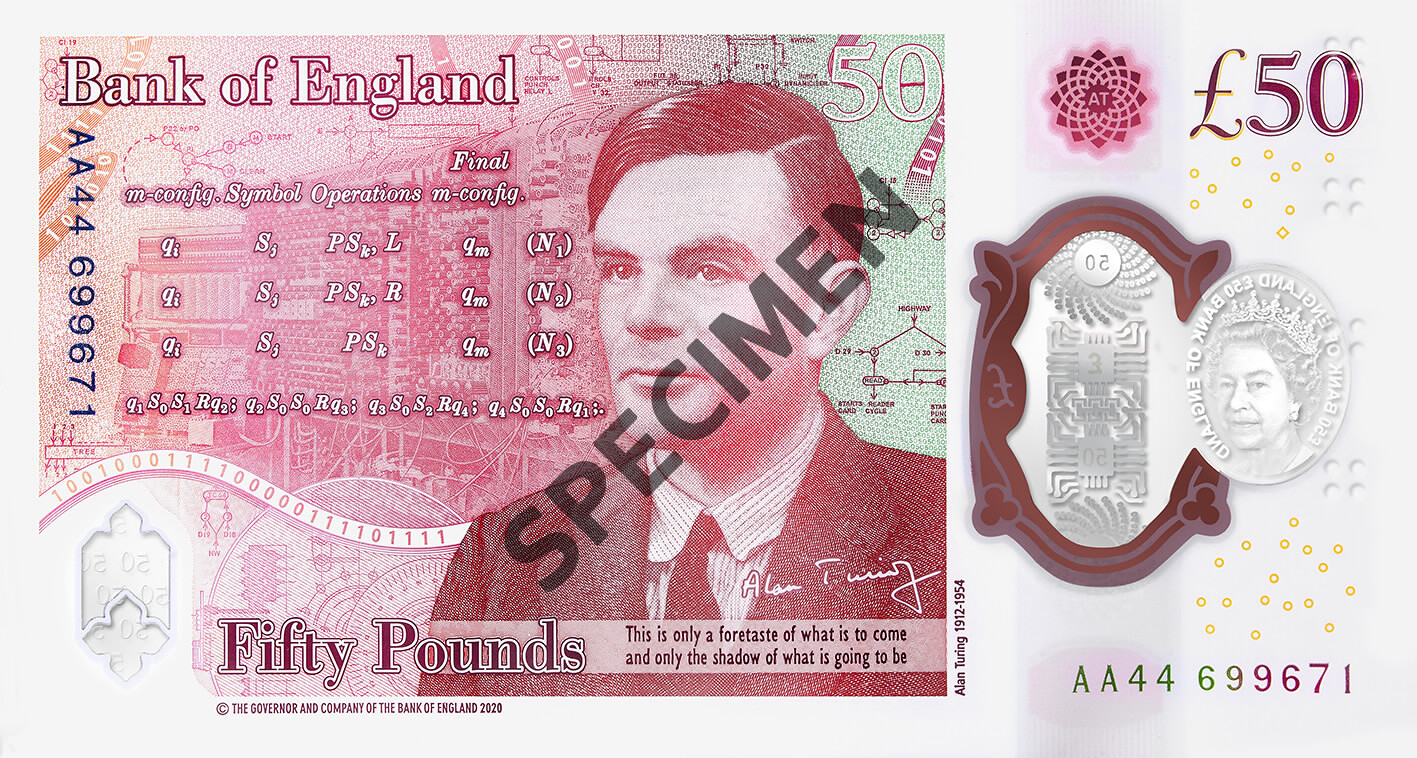
\includegraphics[scale=1]{Turing50note.jpg}\\
{\footnotesize(이미지 출처:
 \url{https://www.bankofengland.co.uk/banknotes/polymer-50-pound-note})}
\caption{2021년부터 발행된 영국 50\textsterling{} 지폐 뒷면의
	앨런 튜링(Alan Turing)\label{fig:Turing50note} }
\end{figure}
지금은 영국 고액권 지폐 인물(그림 \ref{fig:Turing50note})인 앨런 튜링에
관해서는 관련 분야 전공자라면 그가 계산이론(theory of computation)의
기초를 놓은 튜링기계(Turing machine)를 고안했으며 그의 이름을 딴
튜링상(A. M. Turing Award)이 컴퓨터 과학 분야의 노벨상에 해당한다는 것을
알 것이다. 그 외에도 튜링 테스트라는 인공지능과 관련된 아이디어나
영화로도 만들어진 세계 제 2차 대전 때 독일군 암호해독 기계를 개발한 것은
대중적으로도 나름 알려져 있다. 그보다 조금 덜 알려진 이야기는 람다계산법을
창시한 알론조 처치가 튜링기계를 고안한 앨런 튜링의 박사학위 지도교수였다는
사실이다. 앨런 튜링을 컴퓨터 과학의 아버지라고 비유하기도 하는데 그런 비유의
연장선에서 알론조 처치를 컴퓨터 과학의 할아버지 정도로 비유할 수 있지 않을까?
앨런 튜링 외에도, 이 책에서 앞서 정규식의 별표 연산을 도입한
스티븐 클레이니(그림 \ref{fig:RegexSynSem})나 지시적 의미구조의 원조 격인
두 사람 중 하나인 데이나 스콧(그림 \ref{fig:StracheyScott})의 지도교수도
알론조 처치다.

\subsection{처치--튜링 명제(Church-Turing thesis)}
논리로 수학의 토대를 놓으려는 시도에 관한 연구하려는 비슷한 목적으로 고안된,
처치의 타입없는 람다계산법은 바꿔치기의 개념으로 표현된 함수를 기반으로 하며
튜링의 튜링기계는 상태를 변화시키는 추상적인 기계를 기반으로 하므로
표면적으로는 상당히 다르게 보인다. 그런데 학위과정의 스승과 제자로 만나
각자의 아이디어를 비교해 보니 똑같은 범위의 `계산'을 다루고 있었다는 것을
알게 되었다고 한다. 대서양 건너편의 미국과 영국에서 두 천재가 비슷한 시기에
비슷한 주제를 놓고 상당히 다르게 보이는 도구를 고안했는데 우연찮게 그 표현
범위가 일치하였고, 이후로도 지금까지 이 범위를 벗어나는 `계산'을 아직 인류는
발견하지 못했다. 그래서 컴퓨터 혹은 기계로 수행할 수 있는 '계산'이란
처치와 튜링이 생각한 그 이상의 것은 아마도 없을 것이라 가정하고 '계산'의
잠정적인 정의를 곧 람다계산법이나 튜링기계가 다룰 수 있는 범위로 보자는
일종의 경험법칙이 바로 ``처치--튜링 명제''이다.
다시 말하자면 아무리 좋은 프로그래밍언어나 컴퓨터를 설계하더라도 좀더 편리하고
빠르게 계산할 수는 있을지언정 람다계산법이나 튜링기계로 못하는 새로운 계산을
할 수는 없다는 이야기다.

처치--튜링 명제를 받아들인다면 프로그래밍언어를 다음의 두 부류로 분류할 수 있다.
첫째 부류는 람다계산법이나 튜링기계와 같은 범위의 모든 계산이 표현가능한 
튜링완전(Turing-complete) 언어이고 둘째 부류는 그보다 적은 범위의 일부 계산만
표현가능한 튜링완전하지 않은 언어다. 튜링완전 언어는 끝나지 않는 계산 등
다양한 내용을 표현할 수 있는 일반적인 재귀나 반복을 허용한다. 하스켈을 비롯한
일반적인 프로그래밍을 위해 설계된 범용(general-purpose) 프로그래밍언어는 대부분
튜링완전하다. 그런데 우리가 흔히 접하는 프로그래밍언어에 비해 문법구조와
의미구조가 너무나 간단한 처치의 타입없는 람다계산법이 어떻게 모든 계산을
표현할 수 있는지, 이 책에서 처치--튜링 명제를 처음 접한 독자라면 상당히
의아할지도 모르겠다. 여기 \ref{sec:lambdaRec}절에서는 타입없는 람다계산법이 충분히 강력하다는
본보기로 계산이 끝나지 않는 람다식과 일반적인 재귀를 표현할 수 있는
고정점(fixpoint)에 대해 알아본다.

\input{ParaPoly}


\chapter{함수에 대한 값계산}
\label{chap:FunEval}
\ref{chap:ArithExpr}장에서는 산술식에 대한 작은걸음 및 큰걸음
동작과정 의미구조에 대해 알아보았다. 대부분 범용 프로그래밍언어는
산술식과 함께 함수도 지원하므로 함수를 포함하는 언어를
다루는 원리에 대해 이해할 필요가 있다. 람다계산법은 함수를 포함하는
가장 단순한 문법구조로 이루어진 프로그래밍언어로 볼 수 있다. 
이번 장에서는 람다계산법의 값계산(evaluation)에 대한 의미구조를 정의하고
이를 하스켈로 옮겨 구현해 보면서
프로그래밍언어에서 함수를 다루는 원리를 알아본다.
\newpage

\section{줄임(reduction)과 값계산(evaluation)의 맥락적 의미구조}
\label{sec:evalSmallStep}
\index{줄임}\index{reduction}%
\index{비결정적 의미구조}\index{nondeterministic semantics}%
\index{작은걸음 의미구조}\index{small-step semantics}%
\index{맥락적 의미구조}\index{contextual semantics}%
앞서 타입없는 람다계산법의 줄임(reduction)을 규정하는
비결정적 작은걸음 의미구조(\ref{sec:UTLChaskell}절의 그림\;\ref{fig:UTLC})를
소개한 바 있다. 이를 ($\eta$규칙은 제외하고) 맥락적 의미구조의 형태로 옮기면
다음과 같다.
\begin{quote}
문법구조\qquad
$e ~::=~ x \;\mid\; \lambda x.e \;\mid\; e~e$

비결정적 줄임의 맥락적 의미구조 \quad
$(\lambda x.e)\;e_2 \xmapsto{~_B~} \{x{\mapsto}e_2\}e$\\[1.25ex]
$\mathcal{E}
	~ ::= ~  \bullet
	\;\mid\; \lambda x.\mathcal{E}
	\;\mid\; \mathcal{E}~e
	\;\mid\; e~\mathcal{E}
\qquad\qquad
\inference{e\xmapsto{~_B~}e'}{\mathcal{E}[e]\xmapsto{~_C~}\mathcal{E}[e']}$
\end{quote}
위 의미구조에서 값계산 맥락(evaluation context)의 정의만 다음과 같이 바꾸면
\begin{quote}
$\mathcal{E} ~::=~ \bullet \;\mid\; \mathcal{E}~e$
\end{quote}
함수 적용을 우선시하는
\index{적용 먼저 값계산|see{call-by-name evaluation}}%
\index{call-by-name evaluation|see{적용 먼저 값계산}}%
`적용 먼저 값계산'(call-by-name evaluation)의 맥락적
의미구조가 된다. 맥락의 정의에서 $\lambda x.\mathcal{E}$가 제외되었으므로
함수요약식의 함수 몸체 부분의 맥락에서는 더 이상 계산이 진행되지 않는다.
또한, $e~\mathcal{E}$도 제외되었으므로 함수적용식에서 오른쪽에 있는
인자 부분의 맥락에서 계산이 진행되지 않는다. 따라서 함수적용식의 왼쪽이
함수요약식인 경우, 즉 $\beta$줄식($\beta$-redex)인 경우,
선택의 여지 없이 $\beta$줄임으로 계산을 진행하도록 결정된다.
적용 먼저 값계산에서 더 이상 계산이 진행되지 않는 값의 형태($v$)는
다음과 같다.
\begin{quote}
\( \begin{array}{ll}
v ~::=~ n \;\mid\; \lambda x.e  &\quad\text{(values)}\\
n ~::=~ x \;\mid\; n~e          &\quad\text{(neutrals)}
\end{array} \)
\qquad
\( \begin{smallmatrix}
\text{주의:}
	&\text{여기서 $n$은 자연수/정수를 나타내는}\hfill\\
	&\text{기호가 아니라 $v$처럼 특정한 형태의}\hfill\\
	&\text{람다식을 나타내는 기호이다.}\hfill
\end{smallmatrix} \)
\end{quote}
함수에 적용되는 인자의 계산을 우선시하는
\index{인자 먼저 값계산|see{call-by-value evaluation}}%
\index{call-by-value evaluation|see{인자 먼저 값계산}}%
`인자 먼저 값계산'(call-by-value evaluation)의 경우에는
인자가 먼저 값으로 계산된 다음 $\beta$줄임이 진행되어야 하므로
값계산 맥락뿐만 아니라 $\beta$규칙도 다음과 같이 바꿔야 한다.
\begin{quote}
$\mathcal{E} ~::=~ \bullet \;\mid\; \mathcal{E}~e \;\mid\; v~\mathcal{E}
\qquad\qquad\qquad~
(\lambda x.e)\;v_2 \xmapsto{~_B~} \{x{\mapsto}v_2\}e$
\end{quote}
인자 먼저 값계산에서 값의 형태($v$)는 다음과 같다.
\begin{quote}
\( \begin{array}{ll}
v ~::=~ n \;\mid\; \lambda x.e  &\quad\text{(values)}\\
n ~::=~ x \;\mid\; n~v          &\quad\text{(neutrals)}
\end{array} \)
\qquad
\( \begin{smallmatrix}
\text{주의:}
	&\text{여기서 $n$은 자연수/정수를 나타내는}\hfill\\
	&\text{기호가 아니라 $v$처럼 특정한 형태의}\hfill\\
	&\text{람다식을 나타내는 기호이다.}\hfill
\end{smallmatrix} \)

\end{quote}
열린식을 제외한 닫힌식만 고려한다면, 타입없는 람다계산법에서
적용 먼저 값계산이든 인자 먼저 값계산이든 값(value)은
함수요약식($\lambda x.e$)의 형태만 가능하다.

\index{적극적 값계산}\index{eager evaluation}%
인자 먼저 값계산을 `적극적 값계산'이라고도 한다.
적용 먼저(call-by-name) 값계산과 대비되는 문맥에서는 
인자 먼저(call-by-value) 값계산,
\index{게으른 값계산}\index{lazy evaluation}%
게으른 값계산(lazy evaluation)과 대비되는 문맥에서는
적극적 값계산(eager evaluation)으로 부르곤 한다.

\section{값계산 환경을 활용한 큰걸음 의미구조}
\label{sec:evalBigStep}
\index{큰걸음 의미구조}\index{big-step semantics}%
람다계산법의 값계산(evaluation)에 대한 맥락적 작은걸음 의미구조는
람다계산법의 줄임(reduction)에 대한 맥락적 작은걸음 의미구조와 관련해
공통점과 차이점이 잘 드러나기 때문에 값계산과 줄임을 같은 관점에서
연관지어 이해할 수 있다는 장점이 있다. 하지만 이렇게 매번 함수 적용을
할 때마다 함수 몸체에서 파라메터 이름을 인자로
\index{치환}\index{substitution}
치환(substitution)하는
방식을 곧이곧대로 프로그래밍언어의 구현으로 옮긴다면 효율적이지 못한
경우가 많다. 예컨대, 조건식과 산술식이 첨가된 다음과 같은 람다식의
값계산 과정을 살펴보자.
\begin{align*}
& (\lambda x.\lambda y.
	\textbf{if}~x<y
	~\textbf{then}~x+x+x+x
	~\textbf{else}~y+y+y+y)~1~2 \\
\text{\scriptsize($x{\mapsto}1$ 5군데)}~\longmapsto~
& (\lambda y.
	\textbf{if}~1<y
	~\textbf{then}~1+1+1+1
	~\textbf{else}~y+y+y+y)~2 \\
\text{\scriptsize($y{\mapsto}2$ 5군데)}~\longmapsto~
& \textbf{if}~1<2
	~\textbf{then}~1+1+1+1
	~\textbf{else}~2+2+2+2 \\ \longmapsto~
& 1+1+1+1 \longmapsto~\cdots~\longmapsto~ 4
\end{align*}
위 계산 과정의 첫째와 둘째 작은걸음에서 $x$를 1로 다섯 군데에서 치환하고
$y$를 2로 다섯 군데에서 치환한다. $x$를 바꿔친 1은 그 이후의 계산 과정에서
실제로 다섯 군데 모두 결과값을 계산하는 데 활용되지만, $y$를 바꿔친 2는
조건식에서 $1<2$를 계산하는 단 한 군데 말고는 활용되지 않는다.
즉, $y+y+y+y$를 $2+2+2+2$로 바꿔쓴 작업은 낭비였다는 말이다.

매번 함수 적용 때마다 식에 나타나는 파라메터 이름을 실제로 바꿔치는 대신
지금까지 치환했어야 할 내용을 한데 모아 놓은 목록을 만들어
$\{ y{\mapsto}2,\,x{\mapsto}1 \}$와 같이 정리해 두고 필요한 곳에서만
참조하여 활용하면 불필요한 치환을 피할 수 있게 되므로 더 효율적일 것이다.
즉, 값계산 과정의 진행에 필요한 $x<y$에서 $y$가 어떤 값인지 딱 한 번만
찾아보면 되므로, 앞서 살펴본 치환 기반의 작은걸음 계산 과정에서
$y+y+y+y$를 $2+2+2+2$로 바꿔쓰는 불필요한 작업을 하지 않아도 된다. 
이렇게 치환 기반의 의미구조에서 치환했어야 할 내용을 차곡차곡 정리해
한데 모아 놓은 것을
\index{값계산 환경|see{evaluation environment}}%
\index{evaluation environment|see{값계산 환경}}%
`값계산 환경'(evaluation environment) 또는
\index{실행 환경|see{evaluation environment}}%
\index{execution environment|see{실행 환경}}%
`실행 환경'(execution environment)이라고도 하는데, 혼동의 여지가 없는
경우에는 줄여서 그냥 `환경'(environment)이라고 부르기도 한다. 지금부터는
값계산 환경을 활용한 큰걸음 의미구조에 대해 좀더 구체적으로 알아보기로 하자.

값계산 환경을 활용한 의미구조에서는 식에 나타나는 이름에 대응되는 값을
환경에서 참조하는 방식으로 계산이 진행되므로 식($e$)과 그 식을 계산하며
참조할 환경($\rho$)을 항상 짝지어 계산을 진행한다. 즉,
큰걸음 관계($\Longmapsto$)의 왼항에 식과 환경의 순서쌍이 오도록
$\langle e,\rho\rangle\Longmapsto v$와 같이 계산한다는 말이다.
그렇다면 오른항에 오는 값 $v$의 형태는 어떠해야 할까? 환경을 활용하는
의미구조에서는 보통 닫힌식의 값계산만을 고려하므로, 타입없는 람다계산법에서
계산이 끝난 것으로 보는 값은 $\lambda x.e$ 형태의 함수요약식 뿐이다.
그런데 값계산 환경을 활용하는 의미구조에서는 함께 순서쌍을 이루어야
하므로 값의 형태는 $\langle\lambda x.e,\rho\rangle$가 된다. 단,
이 때 $\lambda x.e$에 나타나는 묶이지 않은 모든 자유이름
$x'\in \mathrm{fv}(\lambda x.e)$를 환경으로부터 $\rho(x')$와
같이 참조할 수 있어야 한다. 환경 $\rho$를 함수로 본다면
그 정의역(domain)에 $\lambda x.e$의 자유이름이 모두 포함되어야 한다는 말이다.

일반적으로 식($e$)에 자유변수가 나타날 수 있어 단독으로 놓고 보면 열린식이지만
환경($\rho$)의 정의역이 이를 모두 덮는 경우 전체 순서쌍을 놓고 보면
마치 닫힌식 같다는 의미에서 그러한 $\langle e,\rho\rangle$를
\index{클로저|see{closure}}\index{closure|see{클로저}}%
`클로저'(closure)라 일컫는다.
참고로, 자바스크립트 등의 언어에서도 중첩된 함수 활용에서 발생하는 현상을
설명하려 클로저의 개념을 동원하기도 한다.\footnote{%
\url{https://developer.mozilla.org/ko/docs/Web/JavaScript/Closures} }



\begin{figure}
\begin{align*}
& &
e\in\texttt{Expr} ::=~& x ~\mid~ \lambda x.e ~\mid~ e\;e
\\[1.5ex]
\texttt{Val} \;\subset~ &
	\texttt{Expr}\times\texttt{Env} &
v\in\texttt{Val} ~::=~& \langle\,\lambda x.e,\,\rho\,\rangle
\quad \text{\footnotesize(\,단, $\mathrm{fv}(\lambda x.e)\subset\mathrm{dom}(\rho)$\,)}
\\
\texttt{Env} \,~=~&
	\texttt{Nm} \xrightharpoonup{\,_\textrm{fin}\,} \texttt{Val} &
\rho\in\texttt{Env} ~::=~& \{\,x_1{\mapsto}v_1,\,\ldots,\,x_k{\mapsto}v_k\,\}
\\[1.5ex]
\cdot\stackrel{\!\!_\textrm{cbv}}{\Longmapsto}\cdot \subset~&
	(\texttt{Expr}\times\texttt{Env}) \times \texttt{Val}
\end{align*}
\vspace*{-2em}
\[
\inference[($x$)]{}{
 \langle x,\rho\rangle \stackrel{\!\!_\textrm{cbv}}{\Longmapsto} \rho(x) }
\qquad\qquad
\inference[($\lambda$)]{}{\langle\lambda x.e,\rho\rangle \stackrel{\!\!_\textrm{cbv}}{\Longmapsto} \langle\lambda x.e,\rho\rangle}
\]
\[
\inference[($@$)]{\langle e_1,\rho\rangle \stackrel{\!\!_\textrm{cbv}}{\Longmapsto} \langle \lambda x.e,\rho_1\rangle
& \langle e_2,\rho\rangle \stackrel{\!\!_\textrm{cbv}}{\Longmapsto} v_2 
& \langle e,\{x{\mapsto}v_2\}\rho_1\rangle \stackrel{\!\!_\textrm{cbv}}{\Longmapsto} v
   }{\langle e_1\;e_2,\rho\rangle \stackrel{\!\!_\textrm{cbv}}{\Longmapsto} v}
\]
\caption{타입없는 람다계산법의 인자 먼저 값계산(call-by-value evaluation)을
	규정하는 큰걸음 의미구조
	\label{fig:bigStepCBV} }
\end{figure}

\begin{figure}
\begin{align*}
& &
e\in\texttt{Expr} ::=~& x ~\mid~ \lambda x.e ~\mid~ e\;e
\\[1.5ex]
\texttt{Val} \;\subset~ &
	\texttt{Expr}\times \texttt{Env} &
v\in\texttt{Val} ~::=~& \langle\,\lambda x.e,\,\rho\,\rangle
\quad \text{\footnotesize(\,단, $\mathrm{fv}(\lambda x.e)\subset\mathrm{dom}(\rho)$\,)}
\\
\texttt{Env} \,~=~&
	\texttt{Nm} \xrightharpoonup{\,_\textrm{fin}\,} \texttt{Expr}\times\texttt{Env} &
\rho\in\texttt{Env} ~::=~& \{\,x_1{\mapsto}\langle e_1,\rho_1\rangle,\,\ldots,\,x_k{\mapsto}\langle e_k,\rho_k\rangle\,\}
\\[1.5ex]
\cdot\stackrel{\!\!_\textrm{cbn}}{\Longmapsto}\cdot \subset~&
	(\texttt{Expr}\times\texttt{Env}) \times \texttt{Val}
\end{align*}
\vspace*{-3ex}
\[
\inference[($x$)]{\rho(x) \stackrel{\!\!_\textrm{cbn}}{\Longmapsto} v}{
	\langle x,\rho\rangle \stackrel{\!\!_\textrm{cbn}}{\Longmapsto} v}
\qquad
\inference[($\lambda$)]{}{
	\langle\lambda x.e,\rho\rangle
	\stackrel{\!\!_\textrm{cbn}}{\Longmapsto}
	\langle\lambda x.e,\rho\rangle }
\]
\[
\inference[($@$)]{
	\langle e_1,\rho\rangle \stackrel{\!\!_\textrm{cbn}}{\Longmapsto}
	\langle\lambda x.e,\rho_1\rangle &
	\langle e,\{x{\mapsto}\langle e_2,\rho\rangle\}\rho_1\rangle
	\stackrel{\!\!_\textrm{cbn}}{\Longmapsto} v}{
	\langle e_1\;e_2,\rho\rangle
	\stackrel{\!\!_\textrm{cbn}}{\Longmapsto} v}
\]
\caption{타입없는 람다계산법의 적용 먼저 값계산(call-by-name evaluation)을
	규정하는 큰걸음 의미구조
	\label{fig:bigStepCBN} }
\end{figure}

타입없는 람다계산법에 대한
\index{인자 먼저 값계산}\index{call-by-value evaluation}%
\index{적용 먼저 값계산}\index{call-by- name evaluation}%
인자 먼저 값계산과 적용 먼저 값계산의
큰걸음 의미구조가 그림 \ref{fig:bigStepCBV}와 \ref{fig:bigStepCBN}에
나타나 있는데 그 차이점을 중심으로 살펴보자. 인자 먼저(call-by-value)
값계산 환경에서는 이름에 항상 계산이 끝마친 상태의 값에 대응되므로
이름에 대한 값계산 규칙($x$)에서 환경의 내용을 참조한 $\rho(x)$가
그대로 결과값이 된다. 반면, 적용 먼저(call-by-name) 값계산 환경에서는 
이름에 값이 아닌 형태의 환경과 람다식의 순서쌍이 대응될 수도 있다.
따라서 이름에 대한 값계산 규칙($x$)에서 환경의 내용을 참조한 $\rho(x)$가
아직 계산이 끝나지 않았을지도 모르므로 $\rho(x)$를 큰걸음으로
진행해 보아야 한다. 함수요약식에 대한 값계산 규칙($\lambda$)은 인자 먼저든
적용 먼저든 차이점이 없다. 함수적용식에 대한 값계산 규칙($@$)에는
각 값계산 전략의 특징이 잘 드러난다. 인자 먼저(call-by-value) 값계산
규칙에서는 인자를 값으로 계산하는 과정($\langle e_2,\rho\rangle \stackrel{\!\!_\textrm{cbv}}{\Longmapsto} v_2$)이 나타나는 반면,
적용 먼저(call-by-name) 값계산 규칙에서는 그런 과정 없이
함수 파라메터($x$)에 인자식($e_2$) 그대로의
클로저($\langle e_2,\rho\rangle$)에 대응시켜
적용하는 함수값의 환경($\rho_1$)을 확장한 환경
($\{x{\mapsto}\langle e_2,\rho\rangle\}\rho_1$)에서 함수 몸체($e$)를 계산한다.

\input{FunEval}

\chapter{함수, 산술식, 조건식을 포함하는 언어에 대한 값계산}\label{chap:FunArithEval}
\input{FunArithEval}
